% Options for packages loaded elsewhere
\PassOptionsToPackage{unicode}{hyperref}
\PassOptionsToPackage{hyphens}{url}
%
\documentclass[
]{article}
\usepackage{amsmath,amssymb}
\usepackage{lmodern}
\usepackage{iftex}
\ifPDFTeX
  \usepackage[T1]{fontenc}
  \usepackage[utf8]{inputenc}
  \usepackage{textcomp} % provide euro and other symbols
\else % if luatex or xetex
  \usepackage{unicode-math}
  \defaultfontfeatures{Scale=MatchLowercase}
  \defaultfontfeatures[\rmfamily]{Ligatures=TeX,Scale=1}
\fi
% Use upquote if available, for straight quotes in verbatim environments
\IfFileExists{upquote.sty}{\usepackage{upquote}}{}
\IfFileExists{microtype.sty}{% use microtype if available
  \usepackage[]{microtype}
  \UseMicrotypeSet[protrusion]{basicmath} % disable protrusion for tt fonts
}{}
\makeatletter
\@ifundefined{KOMAClassName}{% if non-KOMA class
  \IfFileExists{parskip.sty}{%
    \usepackage{parskip}
  }{% else
    \setlength{\parindent}{0pt}
    \setlength{\parskip}{6pt plus 2pt minus 1pt}}
}{% if KOMA class
  \KOMAoptions{parskip=half}}
\makeatother
\usepackage{xcolor}
\IfFileExists{xurl.sty}{\usepackage{xurl}}{} % add URL line breaks if available
\IfFileExists{bookmark.sty}{\usepackage{bookmark}}{\usepackage{hyperref}}
\hypersetup{
  pdftitle={Gene\_expression\_analysis},
  pdfauthor={Fay},
  hidelinks,
  pdfcreator={LaTeX via pandoc}}
\urlstyle{same} % disable monospaced font for URLs
\usepackage[margin=1in]{geometry}
\usepackage{color}
\usepackage{fancyvrb}
\newcommand{\VerbBar}{|}
\newcommand{\VERB}{\Verb[commandchars=\\\{\}]}
\DefineVerbatimEnvironment{Highlighting}{Verbatim}{commandchars=\\\{\}}
% Add ',fontsize=\small' for more characters per line
\usepackage{framed}
\definecolor{shadecolor}{RGB}{248,248,248}
\newenvironment{Shaded}{\begin{snugshade}}{\end{snugshade}}
\newcommand{\AlertTok}[1]{\textcolor[rgb]{0.94,0.16,0.16}{#1}}
\newcommand{\AnnotationTok}[1]{\textcolor[rgb]{0.56,0.35,0.01}{\textbf{\textit{#1}}}}
\newcommand{\AttributeTok}[1]{\textcolor[rgb]{0.77,0.63,0.00}{#1}}
\newcommand{\BaseNTok}[1]{\textcolor[rgb]{0.00,0.00,0.81}{#1}}
\newcommand{\BuiltInTok}[1]{#1}
\newcommand{\CharTok}[1]{\textcolor[rgb]{0.31,0.60,0.02}{#1}}
\newcommand{\CommentTok}[1]{\textcolor[rgb]{0.56,0.35,0.01}{\textit{#1}}}
\newcommand{\CommentVarTok}[1]{\textcolor[rgb]{0.56,0.35,0.01}{\textbf{\textit{#1}}}}
\newcommand{\ConstantTok}[1]{\textcolor[rgb]{0.00,0.00,0.00}{#1}}
\newcommand{\ControlFlowTok}[1]{\textcolor[rgb]{0.13,0.29,0.53}{\textbf{#1}}}
\newcommand{\DataTypeTok}[1]{\textcolor[rgb]{0.13,0.29,0.53}{#1}}
\newcommand{\DecValTok}[1]{\textcolor[rgb]{0.00,0.00,0.81}{#1}}
\newcommand{\DocumentationTok}[1]{\textcolor[rgb]{0.56,0.35,0.01}{\textbf{\textit{#1}}}}
\newcommand{\ErrorTok}[1]{\textcolor[rgb]{0.64,0.00,0.00}{\textbf{#1}}}
\newcommand{\ExtensionTok}[1]{#1}
\newcommand{\FloatTok}[1]{\textcolor[rgb]{0.00,0.00,0.81}{#1}}
\newcommand{\FunctionTok}[1]{\textcolor[rgb]{0.00,0.00,0.00}{#1}}
\newcommand{\ImportTok}[1]{#1}
\newcommand{\InformationTok}[1]{\textcolor[rgb]{0.56,0.35,0.01}{\textbf{\textit{#1}}}}
\newcommand{\KeywordTok}[1]{\textcolor[rgb]{0.13,0.29,0.53}{\textbf{#1}}}
\newcommand{\NormalTok}[1]{#1}
\newcommand{\OperatorTok}[1]{\textcolor[rgb]{0.81,0.36,0.00}{\textbf{#1}}}
\newcommand{\OtherTok}[1]{\textcolor[rgb]{0.56,0.35,0.01}{#1}}
\newcommand{\PreprocessorTok}[1]{\textcolor[rgb]{0.56,0.35,0.01}{\textit{#1}}}
\newcommand{\RegionMarkerTok}[1]{#1}
\newcommand{\SpecialCharTok}[1]{\textcolor[rgb]{0.00,0.00,0.00}{#1}}
\newcommand{\SpecialStringTok}[1]{\textcolor[rgb]{0.31,0.60,0.02}{#1}}
\newcommand{\StringTok}[1]{\textcolor[rgb]{0.31,0.60,0.02}{#1}}
\newcommand{\VariableTok}[1]{\textcolor[rgb]{0.00,0.00,0.00}{#1}}
\newcommand{\VerbatimStringTok}[1]{\textcolor[rgb]{0.31,0.60,0.02}{#1}}
\newcommand{\WarningTok}[1]{\textcolor[rgb]{0.56,0.35,0.01}{\textbf{\textit{#1}}}}
\usepackage{graphicx}
\makeatletter
\def\maxwidth{\ifdim\Gin@nat@width>\linewidth\linewidth\else\Gin@nat@width\fi}
\def\maxheight{\ifdim\Gin@nat@height>\textheight\textheight\else\Gin@nat@height\fi}
\makeatother
% Scale images if necessary, so that they will not overflow the page
% margins by default, and it is still possible to overwrite the defaults
% using explicit options in \includegraphics[width, height, ...]{}
\setkeys{Gin}{width=\maxwidth,height=\maxheight,keepaspectratio}
% Set default figure placement to htbp
\makeatletter
\def\fps@figure{htbp}
\makeatother
\setlength{\emergencystretch}{3em} % prevent overfull lines
\providecommand{\tightlist}{%
  \setlength{\itemsep}{0pt}\setlength{\parskip}{0pt}}
\setcounter{secnumdepth}{-\maxdimen} % remove section numbering
\ifLuaTeX
  \usepackage{selnolig}  % disable illegal ligatures
\fi

\title{Gene\_expression\_analysis}
\author{Fay}
\date{2022-05-18}

\begin{document}
\maketitle

GAPDH HKG\\
B-actin HKG\\
Ppia HKG\\
Ppip HKG\\
CDC42 HKG susceptible to DNA contamination

Housekeeping genes selected: GAPDH and PPIB

Relm-b mucosal defense factor (goblet cells)\\
Muc2 the major secretory mucin within the gastrointestinal tract\\
TFF3 mucosal defense factor (goblet cells)\\
Muc5ac similar to MUC2, produced by surface goblet cells\\
NKp46 NK marker\\
F4/80 macropahge marker (distinguish by immune response trend)\\
Mpo myeloperoxidase in Neutrophils\\
MyD88 TLR protein, NF-kB IRAK protein, inflammation marker by TLR
MyD88-Dependent Pathway caspase-1 inflammasome marker (IL-1b and IL-18
production)\\
IL-1Ra natuaral IL-1b antagonist for infection control (if not increase
in Tregs is seen)\\
CXCL9, immune cell migration marker + Th1 activator (confirm FACS)\\
CXCR3, CXCL9 and CXCL11 receptor\\
IL-6 TNF inhibitor,\\
IL-12ra T-cell marker Th1\\
IFN-y compare with IFN-y producing cells and IFN-y ELISAs, should
correlate wit PRF1, NKp46 and F4/80. One of these cell types just have
to be doing the job!\\
IRG6A autonomous cell defense (opsonization)\\
TNF-a upregulated in eimeria but not well explained. Could be present
and driving infection where IFN-y isn't\\
IL-17 in case IFN-y isn't coming up but pathogenicity is\\
TRIF Type I IFN production TRIF Dependent Pathway\\
Socs1 JAK/STAT signaling pathway, proinflammatory regulating + T-cell
differentiation, could explain severity\\
IDO1 DC, monocyte and MC protein regulating T-cell activity\\
Prf1 perforin, should be dominant in primary infections, but must be
correlated between T-cell and NK cell expresions\\
CD56 CD56bright = more cytokine producing NKs, CD56dim = more direct
cytotoxic killing\\
IL-4\\
IL-13\\
IL-10

\hypertarget{gene-expression-in-the-laboratory-infections---heatmap}{%
\subsection{1. Gene expression in the laboratory infections -
Heatmap}\label{gene-expression-in-the-laboratory-infections---heatmap}}

\#document gene normalization
\url{https://www.youtube.com/watch?v=tgp4bbnj-ng} paper: Licak Analysis
of relative gene expression data using real time quantitative Add the
normalized Gene expression to the rest of the data

\url{https://www.youtube.com/watch?v=tgp4bbnj-ng}

If you don't need a graph with absolute values of expressions and just
relative comparison then you can choose one of the samples as a
calibrator (control sample). This control sample will have the value of
1 and the rest of the samples will be compared relative to this one. I
would choose as control the sample with the lowest expression.

\url{https://www.researchgate.net/post/How-can-I-analyze-qPCR-data-without-control-sample}

\begin{Shaded}
\begin{Highlighting}[]
\CommentTok{\#create calibrator samples for the analysis}
\CommentTok{\# create new columns with the minimum of each gene}
\CommentTok{\# which I will use as the calibrator sample}
\CommentTok{\#create a function which gives you the PPIB value for the minimum value of a gene}
\NormalTok{Dct\_Calibrator }\OtherTok{\textless{}{-}} \ControlFlowTok{function}\NormalTok{(x) \{}
\NormalTok{ h }\OtherTok{\textless{}{-}}\NormalTok{  gene[}\FunctionTok{which}\NormalTok{(gene[[x]] }\SpecialCharTok{==} \FunctionTok{min}\NormalTok{(gene[[x]], }\AttributeTok{na.rm =} \ConstantTok{TRUE}\NormalTok{)), ][,}\FunctionTok{c}\NormalTok{(x, }\StringTok{"PPIB"}\NormalTok{)]}
\NormalTok{ h[[x]] }\SpecialCharTok{{-}}\NormalTok{ h[[}\StringTok{"PPIB"}\NormalTok{]]}
\NormalTok{\}}


\CommentTok{\#Apply the function to all genes}
\NormalTok{Calibrator\_values }\OtherTok{\textless{}{-}} \FunctionTok{as.data.frame}\NormalTok{(}\FunctionTok{unlist}\NormalTok{(}\FunctionTok{lapply}\NormalTok{(Genes, Dct\_Calibrator)))}

\NormalTok{Calibrator\_values }\OtherTok{\textless{}{-}} \FunctionTok{cbind}\NormalTok{(Calibrator\_values, }\FunctionTok{as.data.frame}\NormalTok{(Genes))}


\NormalTok{Calibrator\_values }\OtherTok{\textless{}{-}}\NormalTok{ Calibrator\_values }\SpecialCharTok{\%\textgreater{}\%}
  \FunctionTok{rename}\NormalTok{(}\AttributeTok{Dct.calibrator =} \StringTok{"unlist(lapply(Genes, Dct\_Calibrator))"}\NormalTok{)}

\NormalTok{Calibrator\_values }\OtherTok{\textless{}{-}}\NormalTok{ Calibrator\_values }\SpecialCharTok{\%\textgreater{}\%} \FunctionTok{pivot\_wider}\NormalTok{(}\AttributeTok{names\_from =}\NormalTok{ Genes, }\AttributeTok{values\_from =}\NormalTok{ Dct.calibrator)}



\NormalTok{gene }\OtherTok{\textless{}{-}}\NormalTok{ gene }\SpecialCharTok{\%\textgreater{}\%}
\NormalTok{  dplyr}\SpecialCharTok{::}\FunctionTok{mutate}\NormalTok{(}\AttributeTok{IFNy\_N =} \DecValTok{2}\SpecialCharTok{\^{}{-}}\NormalTok{ ((IFNy }\SpecialCharTok{{-}}\NormalTok{ PPIB) }\SpecialCharTok{{-}}\NormalTok{ Calibrator\_values[[}\StringTok{"IFNy"}\NormalTok{]]),}
                \AttributeTok{CXCR3\_bio\_N  =} \DecValTok{2}\SpecialCharTok{\^{}{-}}\NormalTok{ ((CXCR3\_bio }\SpecialCharTok{{-}}\NormalTok{ PPIB)}\SpecialCharTok{{-}}\NormalTok{ Calibrator\_values[[}\StringTok{"CXCR3\_bio"}\NormalTok{]]),}
                \AttributeTok{IL.6\_N =} \DecValTok{2}\SpecialCharTok{\^{}{-}}\NormalTok{((IL}\FloatTok{.6} \SpecialCharTok{{-}}\NormalTok{ PPIB)}\SpecialCharTok{{-}}\NormalTok{ Calibrator\_values[[}\StringTok{"IL.6"}\NormalTok{]]),}
                \AttributeTok{IL.10\_N =} \DecValTok{2}\SpecialCharTok{\^{}{-}}\NormalTok{((IL}\FloatTok{.10} \SpecialCharTok{{-}}\NormalTok{ PPIB)}\SpecialCharTok{{-}}\NormalTok{ Calibrator\_values[[}\StringTok{"IL.10"}\NormalTok{]]),}
                \AttributeTok{IL.13\_N =} \DecValTok{2}\SpecialCharTok{\^{}{-}}\NormalTok{((IL}\FloatTok{.13} \SpecialCharTok{{-}}\NormalTok{ PPIB)}\SpecialCharTok{{-}}\NormalTok{ Calibrator\_values[[}\StringTok{"IL.13"}\NormalTok{]]),}
                \AttributeTok{IL1RN\_N =} \DecValTok{2}\SpecialCharTok{\^{}{-}}\NormalTok{((IL1RN }\SpecialCharTok{{-}}\NormalTok{ PPIB)}\SpecialCharTok{{-}}\NormalTok{ Calibrator\_values[[}\StringTok{"IL1RN"}\NormalTok{]]),}
                \AttributeTok{CASP1\_N =} \DecValTok{2}\SpecialCharTok{\^{}{-}}\NormalTok{((CASP1 }\SpecialCharTok{{-}}\NormalTok{ PPIB)}\SpecialCharTok{{-}}\NormalTok{ Calibrator\_values[[}\StringTok{"CASP1"}\NormalTok{]]),}
                \AttributeTok{CXCL9\_N  =} \DecValTok{2}\SpecialCharTok{\^{}{-}}\NormalTok{((CXCL9 }\SpecialCharTok{{-}}\NormalTok{ PPIB)}\SpecialCharTok{{-}}\NormalTok{ Calibrator\_values[[}\StringTok{"CXCL9"}\NormalTok{]]),}
                \AttributeTok{IDO1\_N =} \DecValTok{2}\SpecialCharTok{\^{}{-}}\NormalTok{((IDO1 }\SpecialCharTok{{-}}\NormalTok{ PPIB)}\SpecialCharTok{{-}}\NormalTok{ Calibrator\_values[[}\StringTok{"IDO1"}\NormalTok{]]),}
                \AttributeTok{IRGM1\_N =} \DecValTok{2}\SpecialCharTok{\^{}{-}}\NormalTok{(( IRGM1 }\SpecialCharTok{{-}}\NormalTok{ PPIB)}\SpecialCharTok{{-}}\NormalTok{ Calibrator\_values[[}\StringTok{"IRGM1"}\NormalTok{]]),}
                \AttributeTok{MPO\_N  =}  \DecValTok{2}\SpecialCharTok{\^{}{-}}\NormalTok{((MPO }\SpecialCharTok{{-}}\NormalTok{ PPIB) }\SpecialCharTok{{-}}\NormalTok{ Calibrator\_values[[}\StringTok{"MPO"}\NormalTok{]]),}
                \AttributeTok{MUC2\_N =} \DecValTok{2}\SpecialCharTok{\^{}{-}}\NormalTok{((MUC2 }\SpecialCharTok{{-}}\NormalTok{ PPIB)}\SpecialCharTok{{-}}\NormalTok{ Calibrator\_values[[}\StringTok{"MUC2"}\NormalTok{]]),}
                \AttributeTok{MUC5AC\_N =} \DecValTok{2}\SpecialCharTok{\^{}{-}}\NormalTok{((MUC5AC }\SpecialCharTok{{-}}\NormalTok{ PPIB)}\SpecialCharTok{{-}}\NormalTok{ Calibrator\_values[[}\StringTok{"MUC5AC"}\NormalTok{]]),}
                \AttributeTok{MYD88\_N  =} \DecValTok{2}\SpecialCharTok{\^{}{-}}\NormalTok{((MYD88 }\SpecialCharTok{{-}}\NormalTok{ PPIB)}\SpecialCharTok{{-}}\NormalTok{ Calibrator\_values[[}\StringTok{"MYD88"}\NormalTok{]]),}
                \AttributeTok{NCR1\_N  =} \DecValTok{2}\SpecialCharTok{\^{}{-}}\NormalTok{((NCR1 }\SpecialCharTok{{-}}\NormalTok{ PPIB)}\SpecialCharTok{{-}}\NormalTok{ Calibrator\_values[[}\StringTok{"NCR1"}\NormalTok{]]),}
                \AttributeTok{PRF1\_N =} \DecValTok{2}\SpecialCharTok{\^{}{-}}\NormalTok{((PRF1 }\SpecialCharTok{{-}}\NormalTok{ PPIB)}\SpecialCharTok{{-}}\NormalTok{ Calibrator\_values[[}\StringTok{"PRF1"}\NormalTok{]]),}
                \AttributeTok{RETNLB\_N =}  \DecValTok{2}\SpecialCharTok{\^{}{-}}\NormalTok{((RETNLB }\SpecialCharTok{{-}}\NormalTok{ PPIB)}\SpecialCharTok{{-}}\NormalTok{ Calibrator\_values[[}\StringTok{"RETNLB"}\NormalTok{]]),}
                \AttributeTok{SOCS1\_N =} \DecValTok{2}\SpecialCharTok{\^{}{-}}\NormalTok{((SOCS1 }\SpecialCharTok{{-}}\NormalTok{ PPIB)}\SpecialCharTok{{-}}\NormalTok{ Calibrator\_values[[}\StringTok{"SOCS1"}\NormalTok{]]),}
                \AttributeTok{TICAM1\_N  =} \DecValTok{2}\SpecialCharTok{\^{}{-}}\NormalTok{((TICAM1 }\SpecialCharTok{{-}}\NormalTok{ PPIB)}\SpecialCharTok{{-}}\NormalTok{ Calibrator\_values[[}\StringTok{"TICAM1"}\NormalTok{]]),}
                \AttributeTok{TNF\_N =} \DecValTok{2}\SpecialCharTok{\^{}{-}}\NormalTok{((TNF }\SpecialCharTok{{-}}\NormalTok{ PPIB) }\SpecialCharTok{{-}}\NormalTok{ Calibrator\_values[[}\StringTok{"TNF"}\NormalTok{]]))}
           

\CommentTok{\#create a new vector for selecting genes}
\NormalTok{genes\_N }\OtherTok{\textless{}{-}} \FunctionTok{c}\NormalTok{(}\StringTok{"IFNy\_N"}\NormalTok{, }\StringTok{"CXCR3\_bio\_N"}\NormalTok{, }\StringTok{"IL.6\_N"}\NormalTok{, }\StringTok{"IL.10\_N"}\NormalTok{, }\StringTok{"IL.13\_N"}\NormalTok{, }\StringTok{"IL1RN\_N"}\NormalTok{, }
           \StringTok{"CASP1\_N"}\NormalTok{, }\StringTok{"CXCL9\_N"}\NormalTok{, }\StringTok{"IDO1\_N"}\NormalTok{, }\StringTok{"IRGM1\_N"}\NormalTok{, }\StringTok{"MPO\_N"}\NormalTok{, }\StringTok{"MUC2\_N"}\NormalTok{, }\StringTok{"MUC5AC\_N"}\NormalTok{, }\StringTok{"MYD88\_N"}\NormalTok{, }
           \StringTok{"NCR1\_N"}\NormalTok{, }\StringTok{"PRF1\_N"}\NormalTok{, }\StringTok{"RETNLB\_N"}\NormalTok{, }\StringTok{"SOCS1\_N"}\NormalTok{, }\StringTok{"TICAM1\_N"}\NormalTok{, }\StringTok{"TNF\_N"}\NormalTok{)}


\NormalTok{gene\_normalized }\OtherTok{\textless{}{-}}\NormalTok{ gene}
\CommentTok{\# turn the data frame into a matrix and transpose it. We want to have each cell }
 \CommentTok{\# type as a row name }
\NormalTok{ gene }\OtherTok{\textless{}{-}} \FunctionTok{t}\NormalTok{(}\FunctionTok{as.matrix}\NormalTok{(gene }\SpecialCharTok{\%\textgreater{}\%}\NormalTok{ dplyr}\SpecialCharTok{::}\FunctionTok{select}\NormalTok{(}\FunctionTok{c}\NormalTok{(EH\_ID, }\FunctionTok{all\_of}\NormalTok{(genes\_N)))))}
 
 \CommentTok{\#switch the matrix back to a data frame format}
\NormalTok{ gene }\OtherTok{\textless{}{-}} \FunctionTok{as.data.frame}\NormalTok{(gene)}
 
 \CommentTok{\# turn the first row into column names}
\NormalTok{ gene }\SpecialCharTok{\%\textgreater{}\%}
     \FunctionTok{row\_to\_names}\NormalTok{(}\AttributeTok{row\_number =} \DecValTok{1}\NormalTok{) }\OtherTok{{-}\textgreater{}}\NormalTok{ heatmap\_data}
 
 \FunctionTok{table}\NormalTok{(}\FunctionTok{rowSums}\NormalTok{(}\FunctionTok{is.na}\NormalTok{(heatmap\_data)) }\SpecialCharTok{==} \FunctionTok{nrow}\NormalTok{(heatmap\_data))}
\end{Highlighting}
\end{Shaded}

\begin{verbatim}
## 
## FALSE  TRUE 
##    19     1
\end{verbatim}

\begin{Shaded}
\begin{Highlighting}[]
 \CommentTok{\# turn the columns to numeric other wise the heatmap function will not work}
\NormalTok{ heatmap\_data[] }\OtherTok{\textless{}{-}} \FunctionTok{lapply}\NormalTok{(heatmap\_data, }\ControlFlowTok{function}\NormalTok{(x) }\FunctionTok{as.numeric}\NormalTok{(}\FunctionTok{as.character}\NormalTok{(x)))}

 \CommentTok{\# remove columns with only NAs }
\NormalTok{ heatmap\_data }\OtherTok{\textless{}{-}} \FunctionTok{Filter}\NormalTok{(}\ControlFlowTok{function}\NormalTok{(x)}\SpecialCharTok{!}\FunctionTok{all}\NormalTok{(}\FunctionTok{is.na}\NormalTok{(x)), heatmap\_data) }
 
 \CommentTok{\#remove rows with only Nas}
\NormalTok{ heatmap\_data }\OtherTok{\textless{}{-}}\NormalTok{  heatmap\_data[, }\FunctionTok{colSums}\NormalTok{(}\FunctionTok{is.na}\NormalTok{(heatmap\_data)) }\SpecialCharTok{!=} \FunctionTok{nrow}\NormalTok{(heatmap\_data)]}


 \DocumentationTok{\#\#\# Prepare the annotation data frame for the heatmap}

 
\NormalTok{annotation\_df }\OtherTok{\textless{}{-}} \FunctionTok{as\_tibble}\NormalTok{(Challenge) }\SpecialCharTok{\%\textgreater{}\%}
\NormalTok{  dplyr}\SpecialCharTok{::}\FunctionTok{filter}\NormalTok{(infection }\SpecialCharTok{==} \StringTok{"challenge"}\NormalTok{, dpi }\SpecialCharTok{==}\NormalTok{ dpi\_max) }\SpecialCharTok{\%\textgreater{}\%}
\NormalTok{  dplyr}\SpecialCharTok{::}\FunctionTok{group\_by}\NormalTok{(EH\_ID) }\SpecialCharTok{\%\textgreater{}\%}
\NormalTok{  dplyr}\SpecialCharTok{::}\FunctionTok{select}\NormalTok{(}\FunctionTok{c}\NormalTok{(}\StringTok{"EH\_ID"}\NormalTok{, }\StringTok{"Parasite\_challenge"}\NormalTok{, }\StringTok{"infection\_history"}\NormalTok{,}\StringTok{"mouse\_strain"}\NormalTok{, }
                  \StringTok{"max\_WL"}\NormalTok{, }\StringTok{"delta"}\NormalTok{, }\StringTok{"hybrid\_status"}\NormalTok{)) }\SpecialCharTok{\%\textgreater{}\%}
\NormalTok{  dplyr}\SpecialCharTok{::}\FunctionTok{filter}\NormalTok{(EH\_ID }\SpecialCharTok{\%in\%} \FunctionTok{colnames}\NormalTok{(heatmap\_data))}
  
\NormalTok{annotation\_df }\OtherTok{\textless{}{-}} \FunctionTok{unique}\NormalTok{(annotation\_df)}
 

\NormalTok{annotation\_df }\OtherTok{\textless{}{-}} \FunctionTok{as.data.frame}\NormalTok{(}\FunctionTok{unique}\NormalTok{(annotation\_df)) }\SpecialCharTok{\%\textgreater{}\%}
\NormalTok{  dplyr}\SpecialCharTok{::}\FunctionTok{select}\NormalTok{(}\SpecialCharTok{{-}}\NormalTok{EH\_ID)}

\DocumentationTok{\#\#\# Prepare the annotation columns for the heatmap}
\FunctionTok{rownames}\NormalTok{(annotation\_df) }\OtherTok{\textless{}{-}}\NormalTok{ annotation\_df}\SpecialCharTok{$}\NormalTok{EH\_ID}


\CommentTok{\# Match the row names to the heatmap data frame}
\FunctionTok{rownames}\NormalTok{(annotation\_df) }\OtherTok{\textless{}{-}} \FunctionTok{colnames}\NormalTok{(heatmap\_data)}
\end{Highlighting}
\end{Shaded}

Heatmap on gene expression data:

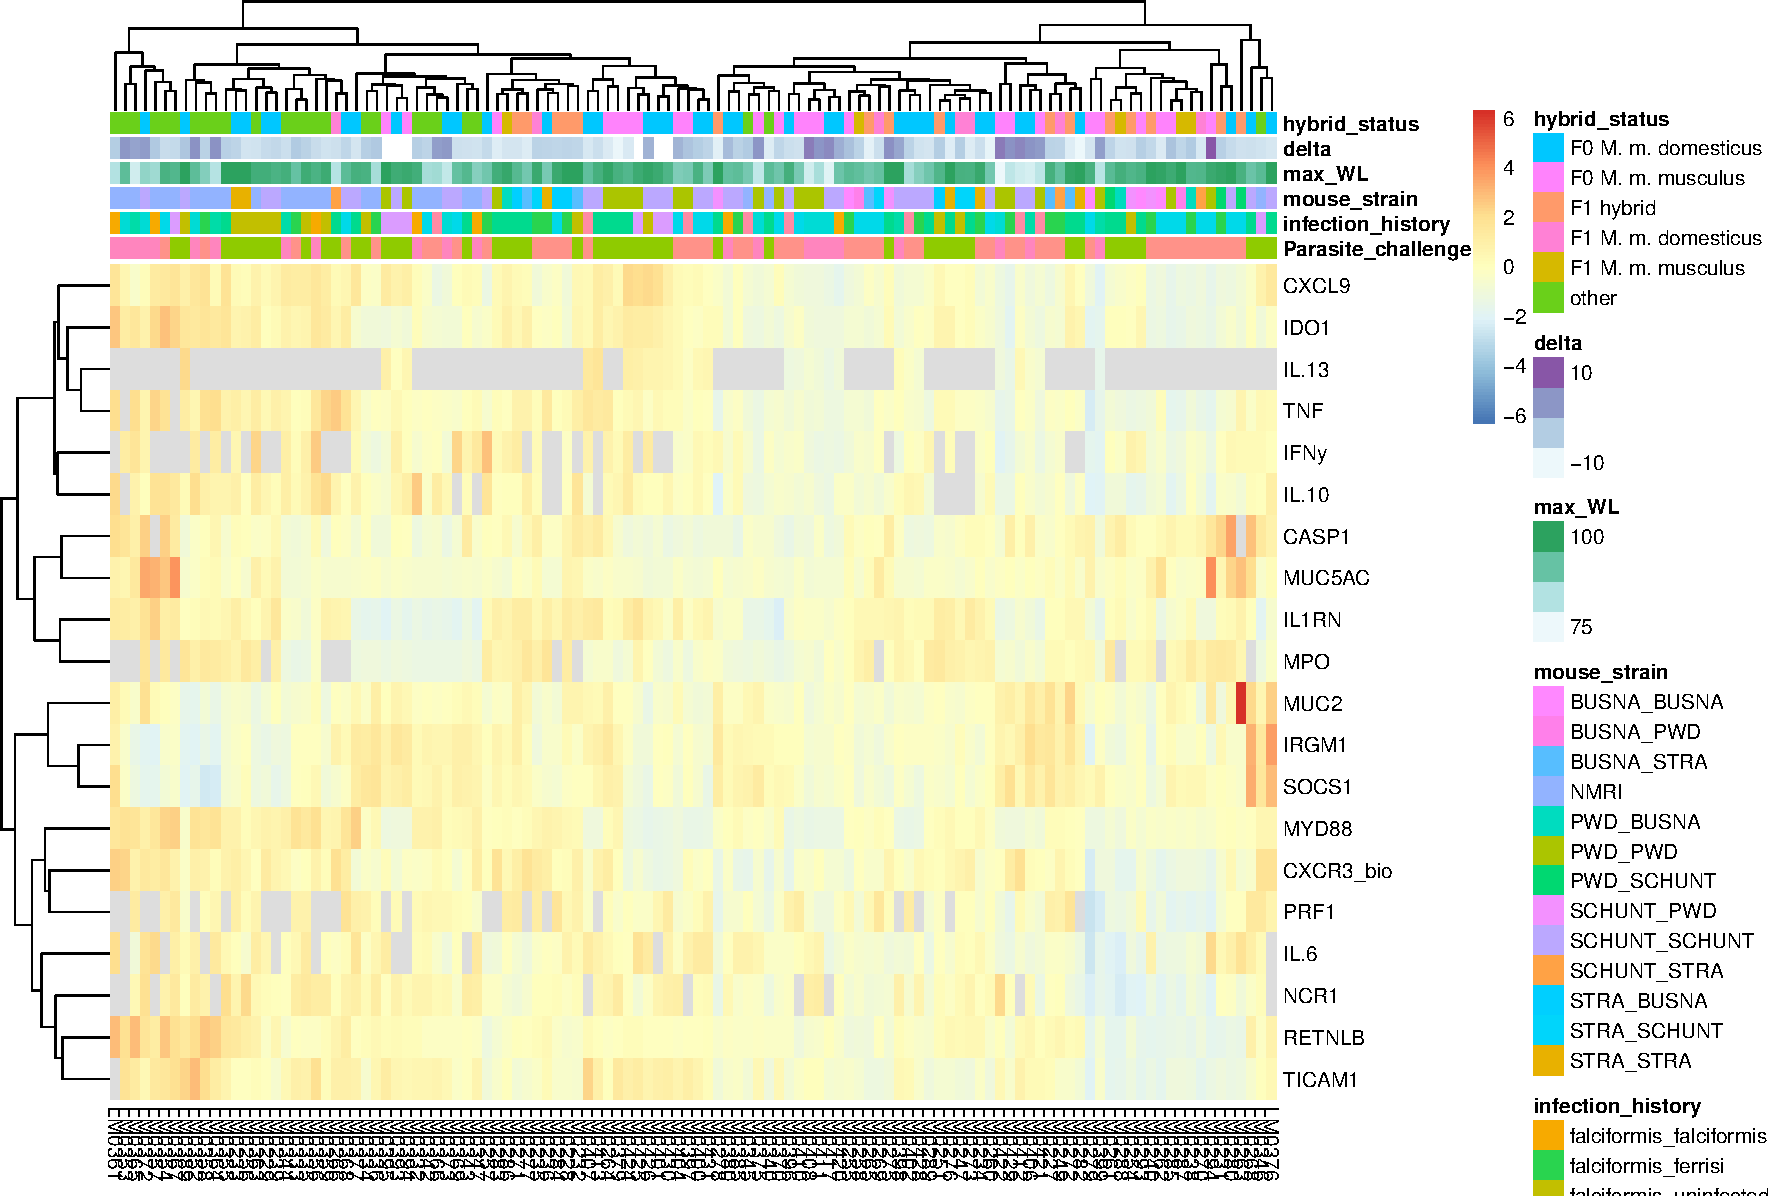
\includegraphics{1.Gene_expression_analysis_files/figure-latex/pheatmap_genes-1.pdf}

\hypertarget{correlations-between-the-genes}{%
\subsection{2. Correlations between the
genes}\label{correlations-between-the-genes}}

\hypertarget{corrplot-of-correlations}{%
\subsection{Corrplot of correlations}\label{corrplot-of-correlations}}

Here is a corrplot of the correlations between the genes. I am using the
non-normalized genes

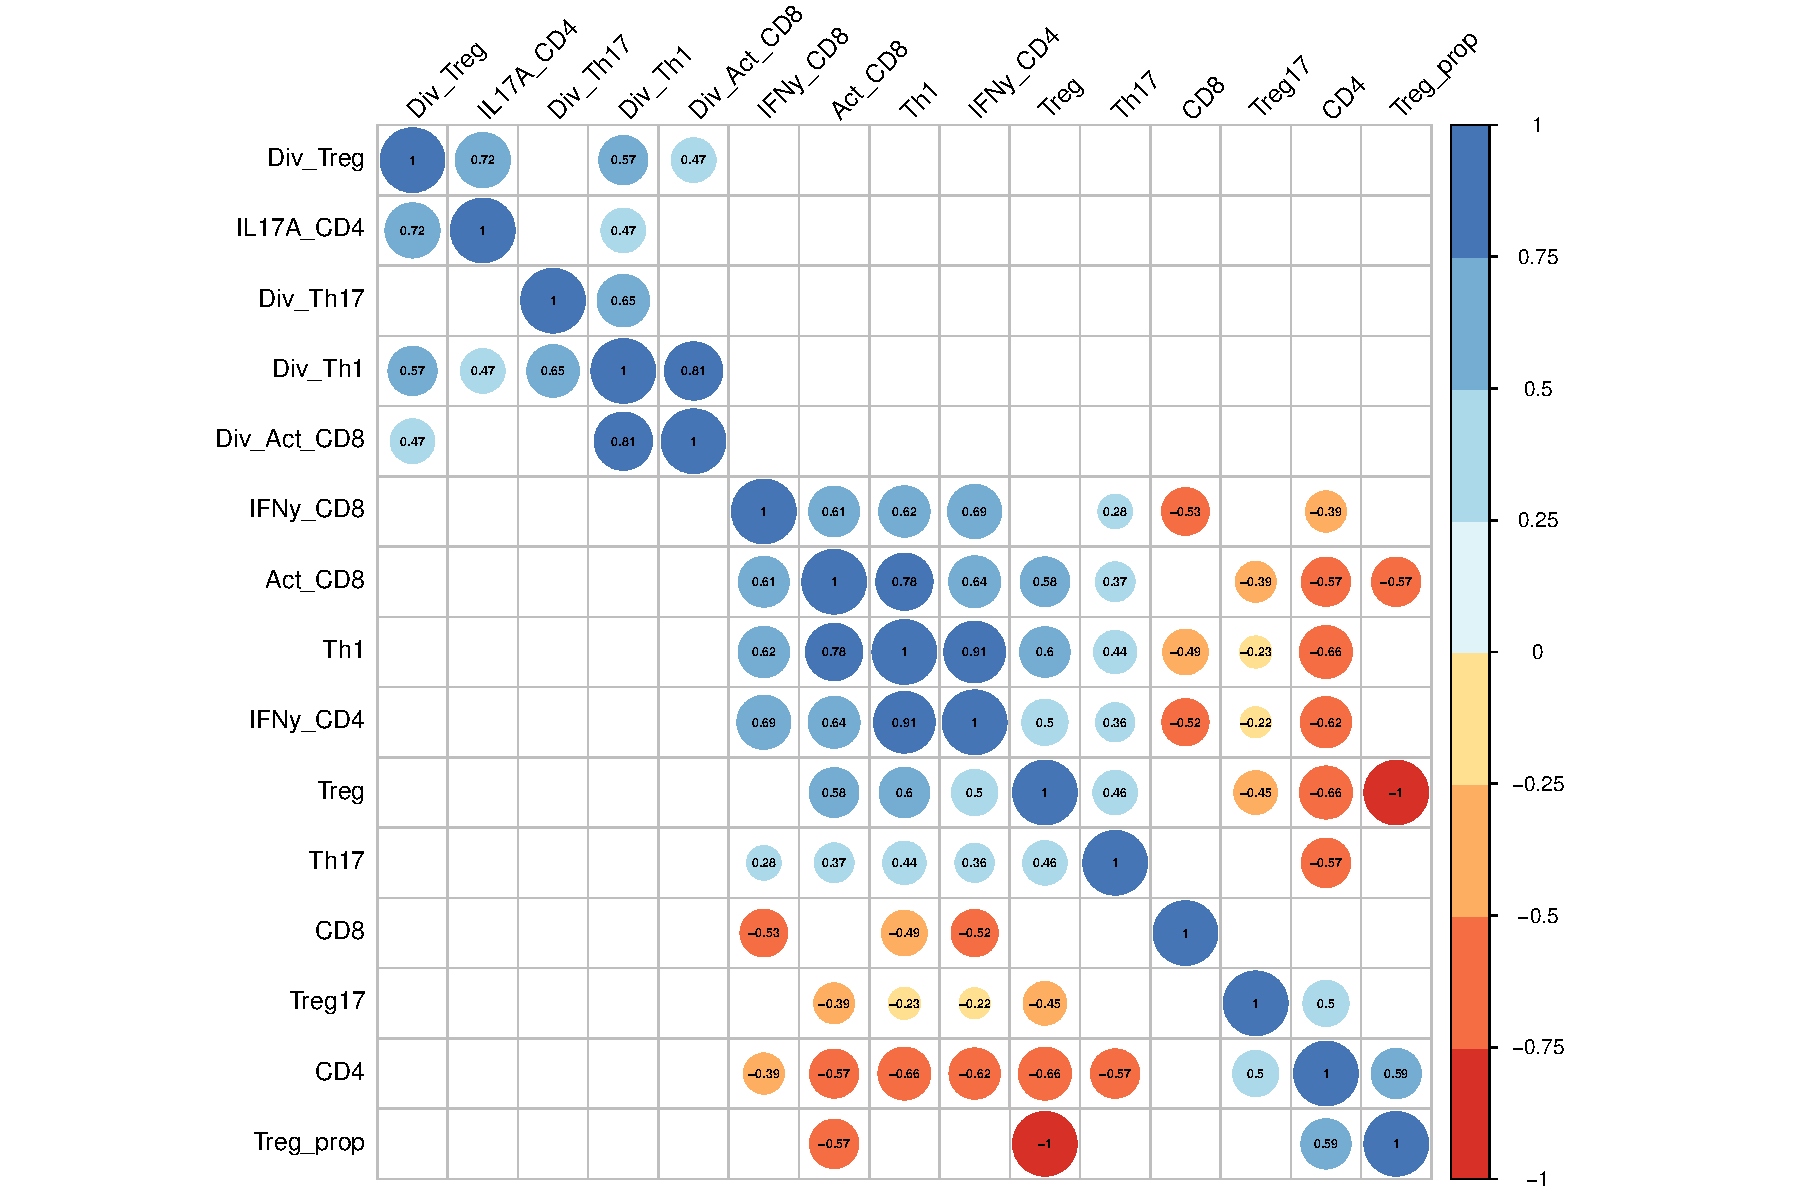
\includegraphics{1.Gene_expression_analysis_files/figure-latex/corrplot_correlations_genes-1.pdf}

\emph{Group 1:}

Muc2 the major secretory mucin within the gastrointestinal tract Mucin 2
is particularly prominent in the gut where it is secreted from goblet
cells in the epithelial lining into the lumen of the large intestine.
There, mucin 2, along with small amounts of related-mucin proteins,
polymerizes into a gel of which 80\% by weight is oligosaccharide
side-chains that are added as post-translational modifications to the
mucin proteins. This gel provides an insoluble mucous barrier that
serves to protect the intestinal epithelium.

IRGM: Immunity-related GTPase family M protein (IRGM), also known as
interferon-inducible protein 1 (IFI1), is an enzyme that in humans is
IRGM gene.{[}5{]}

IRGM is a member of the interferon-inducible GTPase family. The encoded
protein may play a role in the innate immune response by regulating
autophagy formation in response to intracellular pathogens.

SOCS1: Suppressor of cytokine signaling 1 is a protein. SSI family
members are cytokine-inducible negative regulators of cytokine
signaling. The expression of this gene can be induced by a subset of
cytokines, including IL2, IL3 erythropoietin (EPO), GM-CSF, and
interferon-gamma (IFN-γ). The protein encoded by this gene functions
downstream of cytokine receptors, and takes part in a negative feedback
loop to attenuate cytokine signaling. Knockout studies in mice suggested
the role of this gene as a modulator of IFN-γ action, which is required
for normal postnatal growth and survival.{[}8{]} JAK/STAT signaling
pathway, proinflammatory regulating + T-cell differentiation, could
explain severity

\emph{Group 2:} IFNy: IFN-γ, or type II interferon, is a cytokine that
is critical for innate and adaptive immunity against viral, some
bacterial and protozoan infections. IFN-γ is an important activator of
macrophages and inducer of major histocompatibility complex class II
molecule expression. Aberrant IFN-γ expression is associated with a
number of autoinflammatory and autoimmune diseases. The importance of
IFN-γ in the immune system stems in part from its ability to inhibit
viral replication directly, and most importantly from its
immunostimulatory and immunomodulatory effects. IFN-γ is produced
predominantly by natural killer cells (NK) and natural killer T cells
(NKT) as part of the innate immune response, and by CD4 Th1 and CD8
cytotoxic T lymphocyte (CTL) effector T cells once antigen-specific
immunity develops{[}11{]}{[}12{]} as part of the adaptive immune
response. IFN-γ is also produced by non-cytotoxic innate lymphoid cells
(ILC), a family of immune cells first discovered in the early
2010s.{[}13{]}

IL10: IL-10 is a cytokine with multiple, pleiotropic, effects in
immunoregulation and inflammation. It downregulates the expression of
Th1 cytokines, MHC class II antigens, and co-stimulatory molecules on
macrophages. It also enhances B cell survival, proliferation, and
antibody production. IL-10 can block NF-κB activity, and is involved in
the regulation of the JAK-STAT signaling pathway. Further investigation
has shown that IL-10 predominantly inhibits lipopolysaccharide (LPS) and
bacterial product mediated induction of the pro-inflammatory cytokines
TNFα,{[}24{]} IL-1β,{[}24{]} IL-12,{[}25{]} and IFNγ{[}26{]} secretion
from Toll-Like Receptor (TLR) triggered myeloid lineage cells. IL-10 is
capable of inhibiting synthesis of pro-inflammatory cytokines such as
IFN-γ, IL-2, IL-3, TNFα and GM-CSF made by cells such as macrophages and
Th1 T cells. It also displays a potent ability to suppress the
antigen-presentation capacity of antigen presenting cells; however, it
is also stimulatory towards certain T cells (Th2) and mast cells and
stimulates B cell maturation and antibody production.

CXCL9: Chemokine (C-X-C motif) ligand 9 (CXCL9) is a small cytokine
belonging to the CXC chemokine family that is also known as monokine
induced by gamma interferon (MIG). The CXCL9 is one of the chemokine
which plays role to induce chemotaxis, promote differentiation and
multiplication of leukocytes, and cause tissue extravasation.{[}3{]}

The CXCL9/CXCR3 receptor regulates immune cell migration,
differentiation, and activation. Immune reactivity occurs through
recruitment of immune cells, such as cytotoxic lymphocytes (CTLs),
natural killer (NK) cells, NKT cells, and macrophages. Th1 polarization
also activates the immune cells in response to IFN-γ.{[}4{]}
Tumor-infiltrating lymphocytes are a key for clinical outcomes and
prediction of the response to checkpoint inhibitors.{[}5{]} In vivo
studies suggest the axis plays a tumorigenic role by increasing tumor
proliferation and metastasis.{[}citation needed{]} CXCL9 predominantly
mediates lymphocytic infiltration to the focal sites and suppresses
tumor growth.{[}6{]}

For immune cell differentiation, some reports show that CXCL9 lead to
Th1 polarization through CXCR3.{[}15{]} In vivo model by Zohar et
al.~showed that CXCL9, drove increased transcription of T-bet and RORγ,
leading to the polarization of Foxp3− type 1 regulatory (Tr1) cells or T
helper 17 (Th17) from naive T cells via STAT1, STAT4, and STAT5
phosphorylation.{[}15{]}

Several studies have shown that tumor associated macrophages (TAMs) play
modulatory activities in the TME, and the CXCL9/CXCR3 axis impacts TAMs
polarization. The TAMs have opposite effects; M1 for anti-tumor
activities, and M2 for pro-tumor activities. Oghumu et al clarified that
CXCR3 deficient mice displayed increased IL-4 production and M2
polarization in a murine breast cancer model, and decreased innate and
immune cell-mediated anti-tumor responses.{[}16{]}

For immune cell activation, CXCL9 stimulate immune cells through Th1
polarization and activation. Th1 cells produce IFN-γ, TNF-α, IL-2 and
enhance anti-tumor immunity by stimulating CTLs, NK cells and
macrophages.{[}17{]} The IFN-γ-dependent immune activation loop also
promotes CXCL9 release.{[}3{]}

IDO1: Indoleamine-pyrrole 2,3-dioxygenase (IDO or INDO EC 1.13.11.52) is
a heme-containing enzyme physiologically expressed in a number of
tissues and cells, such as the small intestine, lungs IDO is an
important molecule in the mechanisms of tolerance and its physiological
functions include the suppression of potentially dangerous inflammatory
processes in the body.{[}15{]} IDO also plays a role in natural defense
against microorganisms. Expression of IDO is induced by
interferon-gamma, which explains why the expression increases during
inflammatory diseases

IL.13: nterleukin 13 (IL-13) is a protein that in humans is encoded by
the IL13 gene.{[}4{]}{[}5{]}{[}6{]} IL-13 was first cloned in 1993 and
is located on chromosome 5q31 with a length of 1.4kb.{[}4{]} It has a
mass of 13 kDa and folds into 4 alpha helical bundles.{[}7{]} The
secondary structural features of IL-13 are similar to that of
Interleukin 4 (IL-4); however it only has 25\% sequence identity to IL-4
and is capable of IL-4 independent signaling.{[}7{]}{[}4{]}{[}8{]} IL-13
is a cytokine secreted by T helper type 2 (Th2) cells, CD4 cells,
natural killer T cell, mast cells, basophils, eosinophils and
nuocytes.{[}7{]} Interleukin-13 is a central regulator in IgE synthesis,
goblet cell hyperplasia, mucus hypersecretion, airway
hyperresponsiveness, fibrosis and chitinase up-regulation.{[}7{]} It is
a mediator of allergic inflammation and different diseases including
asthma.{[}7{]} IL-13 specifically induces physiological changes in
parasitized organs that are required to expel the offending organisms or
their products. For example, expulsion from the gut of a variety of
mouse helminths requires IL-13 secreted by Th2 cells. IL-13 induces
several changes in the gut that create an environment hostile to the
parasite, including enhanced contractions and glycoprotein
hyper-secretion from gut epithelial cells, that ultimately lead to
detachment of the organism from the gut wall and their removal.{[}13{]}

TNF: Tumor necrosis factor (TNF, cachexin, or cachectin; often called
tumor necrosis factor alpha or TNF-α) is an adipokine and a cytokine.
TNF is a member of the TNF superfamily, which consists of various
transmembrane proteins with a homologous TNF domain. The primary role of
TNF is in the regulation of immune cells. TNF, as an endogenous pyrogen,
is able to induce fever, apoptotic cell death, cachexia, and
inflammation, inhibit tumorigenesis and viral replication, and respond
to sepsis via IL-1 and IL-6-producing cells. Dysregulation of TNF
production has been implicated in a variety of human diseases including
Alzheimer's disease,{[}12{]} cancer,{[}13{]} major depression,{[}14{]}
psoriasis{[}15{]} and inflammatory bowel disease (IBD).{[}16{]} Though
controversial, some studies have linked depression and IBD to increased
levels of TNF.{[}17{]}{[}18{]} it is produced also by a broad variety of
cell types including lymphoid cells, mast cells, endothelial cells,
cardiac myocytes, adipose tissue, fibroblasts, and
neurons.{[}51{]}{[}unreliable medical source?{]} Large amounts of TNF
are released in response to lipopolysaccharide, other bacterial
products, and interleukin-1 (IL-1). In the skin, mast cells appear to be
the predominant source of pre-formed TNF, which can be released upon
inflammatory stimulus (e.g., LPS).{[}52{]}

TNF promotes the inflammatory response, which, in turn, causes many of
the clinical problems associated with autoimmune disorders such as
rheumatoid arthritis, ankylosing spondylitis, inflammatory bowel
disease, psoriasis, hidradenitis suppurativa and refractory asthma.
These disorders are sometimes treated by using a TNF inhibitor.

\emph{Group 3:} IL1 RN: interleukin 1 receptor antagonist The
interleukin-1 receptor antagonist (IL-1RA) is a protein that in humans
is encoded by the IL1RN gene.{[} IL-1RA is a member of the interleukin 1
cytokine family. IL1Ra is secreted by various types of cells including
immune cells, epithelial cells, and adipocytes, and is a natural
inhibitor of the pro-inflammatory effect of IL1β.{[}8{]} This protein
inhibits the activities of interleukin 1, alpha (IL1A) and interleukin
1, beta (IL1B), and modulates a variety of interleukin 1 related immune
and inflammatory responses.

MPO: Myeloperoxidase (MPO) is a peroxidase enzyme that in humans is
encoded by the MPO gene on chromosome 17.{[}5{]} MPO is most abundantly
expressed in neutrophil granulocytes (a subtype of white blood cells),
and produces hypohalous acids to carry out their antimicrobial activity,
including hypochlorous acid, the sodium salt of which is the chemical in
bleach.{[}5{]}{[}6{]} It is a lysosomal protein stored in azurophilic
granules of the neutrophil and released into the extracellular space
during degranulation.{[}7{]} Neutrophil myeloperoxidase has a heme
pigment, which causes its green color in secretions rich in neutrophils,
such as mucus and sputum.{[}8{]} The green color contributed to its
outdated name verdoperoxidase.

MPO is a member of the XPO subfamily of peroxidases and produces
hypochlorous acid (HOCl) from hydrogen peroxide (H2O2) and chloride
anion (Cl−) (or hypobromous acid if Br- is present) during the
neutrophil's respiratory burst. It requires heme as a cofactor.
Furthermore, it oxidizes tyrosine to tyrosyl radical using hydrogen
peroxide as an oxidizing agent.{[}10{]}{[}14{]} Hypochlorous acid and
tyrosyl radical are cytotoxic, so they are used by the neutrophil to
kill bacteria and other pathogens.{[}15{]} However, this hypochlorous
acid may also cause oxidative damage in host tissue. Moreover, MPO
oxidation of apoA-I reduces HDL-mediated inhibition of apoptosis and
inflammation.{[}16{]} In addition, MPO mediates protein nitrosylation
and the formation of 3-chlorotyrosine and dityrosine crosslinks.{[}10{]}

\emph{Group 4:} CASP1: Caspase-1/Interleukin-1 converting enzyme (ICE)
is an evolutionarily conserved enzyme that proteolytically cleaves other
proteins, such as the precursors of the inflammatory cytokines
interleukin 1β and interleukin 18 as well as the pyroptosis inducer
Gasdermin D, into active mature peptides.{[}5{]}{[}6{]}{[}7{]} It plays
a central role in cell immunity as an inflammatory response initiator.
Once activated through formation of an inflammasome complex, it
initiates a proinflammatory response through the cleavage and thus
activation of the two inflammatory cytokines, interleukin 1β (IL-1β) and
interleukin 18 (IL-18) as well as pyroptosis, a programmed lytic cell
death pathway, through cleavage of Gasdermin D.{[}8{]} The two
inflammatory cytokines activated by Caspase-1 are excreted from the cell
to further induce the inflammatory response in neighboring cells.{[}9{]}

MUC5AC: Mucin 5AC (Muc5AC) is a protein that in humans is encoded by the
MUC5AC gene.{[}5{]}{[}6{]}{[}7{]}

Muc5AC is a large gel-forming glycoprotein. In the respiratory tract it
protects against infection by binding to inhaled pathogens that are
subsequently removed by mucociliary clearance. Overproduction of Muc5AC
can contribute to diseases such as asthma and chronic obstructive
pulmonary disease,{[}8{]} and has also been associated with greater
protection against influenza infection.{[}9{]}

\emph{Group 5:} PRF1: Perforin-1 is a protein that in humans is encoded
by the PRF1 gene and the Prf1 gene in mice. Perforin is a pore forming
cytolytic protein found in the granules of cytotoxic T lymphocytes
(CTLs) and natural killer cells (NK cells). Upon degranulation, perforin
molecules translocate to the target cell with the help of calreticulin,
which works as a chaperone protein to prevent perforin from degrading.
Perforin then binds to the target cell's plasma membrane via membrane
phospholipids while phosphatidylcholine binds calcium ions to increase
perforin's affinity to the membrane.{[}8{]} Perforin oligomerises in a
Ca2+ dependent manner to form pores on the target cell. The pore formed
allows for the passive diffusion of a family of pro-apoptotic proteases,
known as the granzymes, into the target cell.{[}9{]} The lytic
membrane-inserting part of perforin is the MACPF domain.{[}10{]} This
region shares homology with cholesterol-dependent cytolysins from
Gram-positive bacteria.{[}11{]}

Perforin has structural and functional similarities to complement
component 9 (C9). Like C9, this protein creates transmembrane tubules
and is capable of lysing non-specifically a variety of target cells.
This protein is one of the main cytolytic proteins of cytolytic
granules, and it is known to be a key effector molecule for T-cell- and
natural killer-cell-mediated cytolysis.{[}7{]} Perforin is thought to
act by creating holes in the plasma membrane which triggers an influx of
calcium and initiates membrane repair mechanisms. These repair
mechanisms bring perforin and granzymes into early endosomes.{[}12{]}

CXCR3: Chemokine receptor CXCR3 is a Gαi protein-coupled receptor in the
CXC chemokine receptor family. Other names for CXCR3 are G
protein-coupled receptor 9 (GPR9) and CD183. There are three isoforms of
CXCR3 in humans: CXCR3-A, CXCR3-B and chemokine receptor 3-alternative
(CXCR3-alt).{[}5{]} CXCR3-A binds to the CXC chemokines CXCL9 (MIG),
CXCL10 (IP-10), and CXCL11 (I-TAC){[}6{]} whereas CXCR3-B can also bind
to CXCL4 in addition to CXCL9, CXCL10, and CXCL11.{[}7{]} CXCR3 is
expressed primarily on activated T lymphocytes and NK cells,{[}8{]} and
some epithelial cells. CXCR3 and CCR5 are preferentially expressed on
Th1 cells, whereas Th2 cells favor the expression of CCR3 and CCR4.
CXCR3 ligands that attract Th1 cells can concomitantly block the
migration of Th2 cells in response to CCR3 ligands, thus enhancing the
polarization of effector T cell recruitment.

MYD88: Myeloid differentiation primary response 88 (MYD88) is a protein
that, in humans, is encoded by the MYD88 gene. Model organisms have been
used in the study of MYD88 function. The gene was originally discovered
and cloned by Dan Liebermann and Barbara Hoffman in mice.{[}7{]} In that
species it is a universal adapter protein as it is used by almost all
TLRs (except TLR 3) to activate the transcription factor NF-κB. Mal
(also known as TIRAP) is necessary to recruit Myd88 to TLR 2 and TLR 4,
and MyD88 then signals through IRAK.{[}8{]} It also interacts
functionally with amyloid formation and behavior in a transgenic mouse
model of Alzheimer's disease.{[}9{]}

Myd88 knockout mouse phenotype A conditional knockout mouse line, called
Myd88tm1a(EUCOMM)Wtsi{[}13{]}{[}14{]} was generated as part of the
International Knockout Mouse Consortium program --- a high-throughput
mutagenesis project to generate and distribute animal models of disease
to interested scientists.{[}15{]}{[}16{]}{[}17{]} Male and female
animals underwent a standardized phenotypic screen to determine the
effects of deletion.{[}11{]}{[}18{]} Twenty-one tests were carried out
on homozygous mutant animals, revealing one abnormality: male mutants
had an increased susceptibility to bacterial infection. The MYD88 gene
provides instructions for making a protein involved in signaling within
immune cells. The MyD88 protein acts as an adapter, connecting proteins
that receive signals from outside the cell to the proteins that relay
signals inside the cell. In innate immunity, the MyD88 plays a pivotal
role in immune cell activation through Toll-like receptors (TLRs), which
belong to large group of pattern recognition receptors (PRR). In
general, these receptors sense common patterns which are shared by
various pathogens -- Pathogen-associated molecular pattern (PAMPs), or
which are produced/released during cellular damage -- damage-associated
molecular patterns (DAMPs).{[}19{]}

IL.6: Interleukin 6 (IL-6) is an interleukin that acts as both a
pro-inflammatory cytokine and an anti-inflammatory myokine. In humans,
it is encoded by the IL6 gene.{[}5{]}

In addition, osteoblasts secrete IL-6 to stimulate osteoclast formation.
Smooth muscle cells in the tunica media of many blood vessels also
produce IL-6 as a pro-inflammatory cytokine. IL-6's role as an
anti-inflammatory myokine is mediated through its inhibitory effects on
TNF-alpha and IL-1 and its activation of IL-1ra and IL-10.

Immune system IL-6 is secreted by macrophages in response to specific
microbial molecules, referred to as pathogen-associated molecular
patterns (PAMPs). These PAMPs bind to an important group of detection
molecules of the innate immune system, called pattern recognition
receptors (PRRs), including Toll-like receptors (TLRs). These are
present on the cell surface and intracellular compartments and induce
intracellular signaling cascades that give rise to inflammatory cytokine
production. IL-6 is an important mediator of fever and of the acute
phase response.

IL-6 is responsible for stimulating acute phase protein synthesis, as
well as the production of neutrophils in the bone marrow. It supports
the growth of B cells and is antagonistic to regulatory T cells.

NCR1: Natural cytotoxicity triggering receptor 1 is a protein that in
humans is encoded by the NCR1 gene.{[}

RETNL:

TICAM1: TIRP is a Toll/interleukin-1 receptor (IL1R; MIM 147810) (TIR)
domain-containing adaptor protein involved in Toll receptor signaling

\begin{verbatim}
## Warning: Removed 115 rows containing missing values (geom_point).
\end{verbatim}

\includegraphics{1.Gene_expression_analysis_files/figure-latex/gene_expression_intensity-1.pdf}

\begin{verbatim}
## Warning: Removed 238 rows containing non-finite values (stat_boxplot).
\end{verbatim}

\begin{verbatim}
## Warning: Removed 238 rows containing missing values (geom_point).
\end{verbatim}

\includegraphics{1.Gene_expression_analysis_files/figure-latex/gene_expression_box-1.pdf}

\begin{verbatim}
## Warning: Ignoring unknown parameters: echo
\end{verbatim}

\begin{verbatim}
## Warning: Removed 238 rows containing non-finite values (stat_bin).
\end{verbatim}

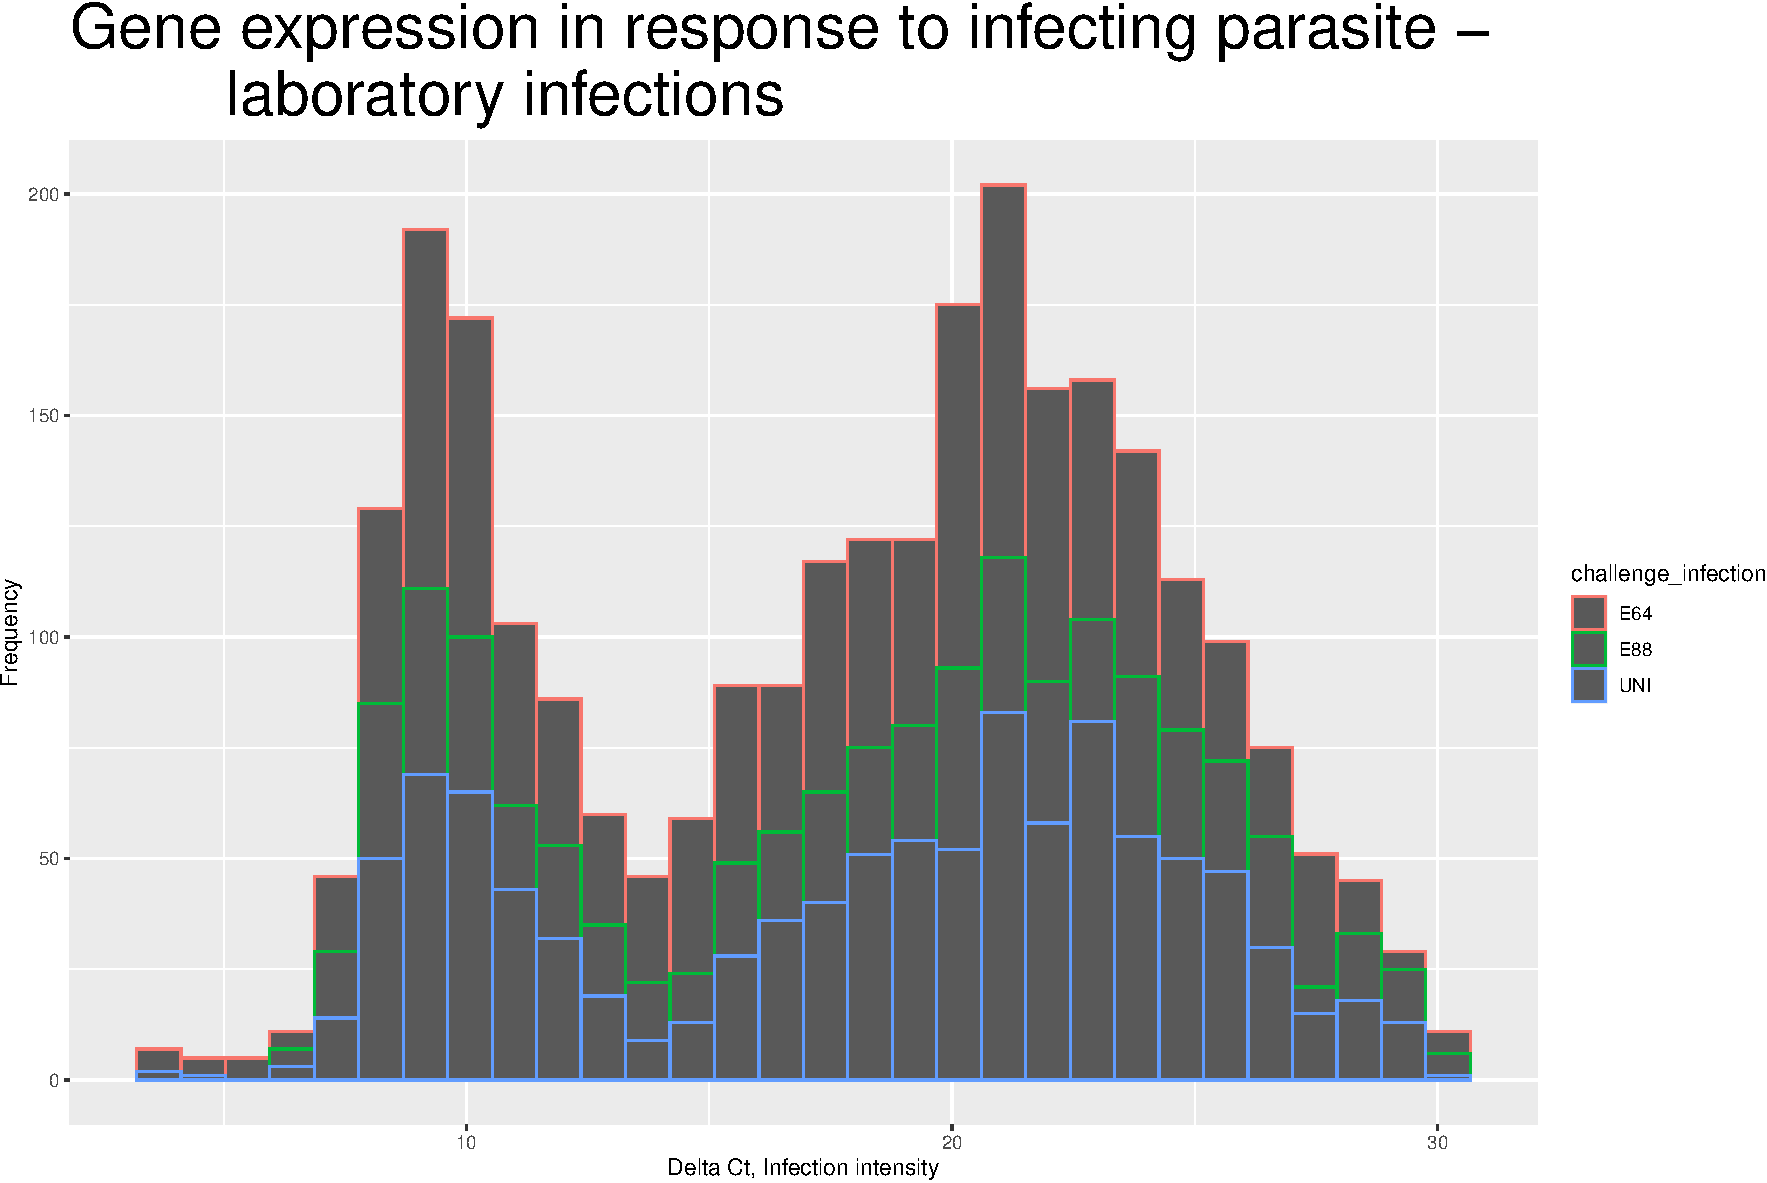
\includegraphics{1.Gene_expression_analysis_files/figure-latex/histogram_genes-1.pdf}

It is possible to compute a pca with missing data using the package
missMDA. The missMDA package is dedicated to missing values in
exploratory multivariate data analysis: single imputation/multiple
imputation, etc.

Following the tutorial of the package author: Francois Husson:
\url{https://www.youtube.com/watch?v=OOM8_FH6_8o}

\hypertarget{pca}{%
\subsection{3. PCA}\label{pca}}

\hypertarget{handling-missing-data-in-a-pca}{%
\paragraph{Handling missing data in a
pca:}\label{handling-missing-data-in-a-pca}}

Bad methods: removing individuals with missing data or replacing missing
data with the mean (default setting in many packages).

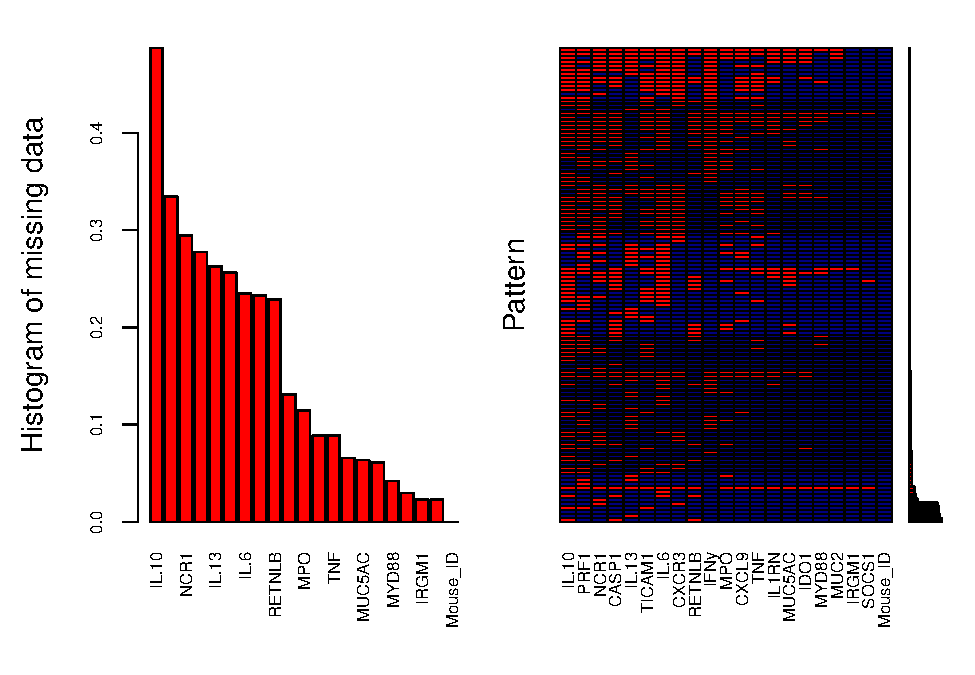
\includegraphics{1.Gene_expression_analysis_files/figure-latex/unnamed-chunk-1-1.pdf}

We will now continue by using an iterative pca to impute missing data A.
Initialization: impute using the mean B. Step lampda: \# a. do pca on
imputed data table S dimensions retained \# b. missing data imputed
using pca \# c.~means (and standard deviations) updated C. Iterate the
estimation and imputation steps (until convergence) (convergence: the
act of converging and especially moving toward union or uniformity)

Overfitting is a common problem due to believing too much in links
between variables. --\textgreater{} regularized iterative PCA (This
version is what is being implented in missMDA) This is a way of taking
less risk when imputing the missing data. The algorithm estimates the
missing data values with values that have no influence on the PCA
results, i.e., no influence on the coordinates of the individals or
variables.

\includegraphics{1.Gene_expression_analysis_files/figure-latex/pca_gene-1.pdf}
\includegraphics{1.Gene_expression_analysis_files/figure-latex/pca_gene-2.pdf}

Caution: When imputing data, the percentages of inertia associated with
the first dimensions will be overestimated.

Another problem: the imputed data are, when the pca is performed
considered like real observations. But they are estimations!!

Visualizing uncertainty due to issing data:

--\textgreater{} mulrimple imputation: generate several plausible values
for each missing data point

We here visualize the variability, that is uncertainty on the plane
defined by two pca axes.

\includegraphics[width=0.5\linewidth]{1.Gene_expression_analysis_files/figure-latex/error_visualization_pca_gene-1}
\includegraphics[width=0.5\linewidth]{1.Gene_expression_analysis_files/figure-latex/error_visualization_pca_gene-2}
\includegraphics[width=0.5\linewidth]{1.Gene_expression_analysis_files/figure-latex/error_visualization_pca_gene-3}
\includegraphics[width=0.5\linewidth]{1.Gene_expression_analysis_files/figure-latex/error_visualization_pca_gene-4}

\begin{verbatim}
## $PlotIndProc
\end{verbatim}

\includegraphics[width=0.5\linewidth]{1.Gene_expression_analysis_files/figure-latex/error_visualization_pca_gene-5}

\begin{verbatim}
## 
## $PlotDim
\end{verbatim}

\includegraphics[width=0.5\linewidth]{1.Gene_expression_analysis_files/figure-latex/error_visualization_pca_gene-6}

\begin{verbatim}
## 
## $PlotIndSupp
\end{verbatim}

\includegraphics[width=0.5\linewidth]{1.Gene_expression_analysis_files/figure-latex/error_visualization_pca_gene-7}

\begin{verbatim}
## 
## $PlotVar
\end{verbatim}

\includegraphics[width=0.5\linewidth]{1.Gene_expression_analysis_files/figure-latex/error_visualization_pca_gene-8}
Individuals lying on the axis have no missing data, but individuals that
far away have many missing data. big ellipse = big uncertainty tight
elipse (line) = low uncertainty

Variable representation: Poins tight together )look like one) - have no
missing variables --\textgreater{} low uncertainty Points spread --
\textgreater{} higher variability -- \textgreater{} higher uncertainty

High uncertainty--\textgreater{} we should interpret the result with
care

The individuals with many missing data values make the axes move, and
thus the positions of all individuals

Therefore in the last plots every individual is getting an eclipse as
they are as well influenced by the missing data of the others.

THe plot with the dimensions shows the projections of the pca dimensions
of each imputed table on the pca plane obtained using the original
imputed data table

As all of the arrows are close to either the first or second axes, this
means that the axes are stable with respect to the set of imputed tables
--\textgreater{} we don't have evidence of instability here.

Biplot of the imputed gene pca

\begin{Shaded}
\begin{Highlighting}[]
\CommentTok{\#Now we can make our initial plot of the PCA.}
\NormalTok{imputed\_expr }\SpecialCharTok{\%\textgreater{}\%} 
  \FunctionTok{pivot\_longer}\NormalTok{(}\AttributeTok{cols =} \FunctionTok{all\_of}\NormalTok{(Genes), }\AttributeTok{names\_to =} \StringTok{"Gene"}\NormalTok{, }\AttributeTok{values\_to =} \StringTok{"gene\_expression"}\NormalTok{)  }\SpecialCharTok{\%\textgreater{}\%}
  \FunctionTok{ggplot}\NormalTok{(}\FunctionTok{aes}\NormalTok{(}\AttributeTok{x =}\NormalTok{ pc1, }\AttributeTok{y =}\NormalTok{ pc2, }\AttributeTok{color =}\NormalTok{ Parasite\_challenge, }\AttributeTok{shape =}\NormalTok{ Parasite\_challenge)) }\SpecialCharTok{+}
  \FunctionTok{geom\_hline}\NormalTok{(}\AttributeTok{yintercept =} \DecValTok{0}\NormalTok{, }\AttributeTok{lty =} \DecValTok{2}\NormalTok{) }\SpecialCharTok{+}
  \FunctionTok{geom\_vline}\NormalTok{(}\AttributeTok{xintercept =} \DecValTok{0}\NormalTok{, }\AttributeTok{lty =} \DecValTok{2}\NormalTok{) }\SpecialCharTok{+}
  \FunctionTok{geom\_point}\NormalTok{(}\AttributeTok{alpha =} \FloatTok{0.8}\NormalTok{) }\SpecialCharTok{+}
  \FunctionTok{stat\_ellipse}\NormalTok{(}\AttributeTok{geom=}\StringTok{"polygon"}\NormalTok{, }\FunctionTok{aes}\NormalTok{(}\AttributeTok{fill =}\NormalTok{ challenge\_infection), }\AttributeTok{alpha =} \FloatTok{0.2}\NormalTok{, }\AttributeTok{show.legend =} \ConstantTok{FALSE}\NormalTok{,}
               \AttributeTok{level =} \FloatTok{0.95}\NormalTok{) }\SpecialCharTok{+}
  \FunctionTok{theme\_minimal}\NormalTok{() }\SpecialCharTok{+}
  \FunctionTok{theme}\NormalTok{(}\AttributeTok{panel.grid =} \FunctionTok{element\_blank}\NormalTok{(), }\AttributeTok{panel.border =} \FunctionTok{element\_rect}\NormalTok{(}\AttributeTok{fill=} \StringTok{"transparent"}\NormalTok{)) }
\end{Highlighting}
\end{Shaded}

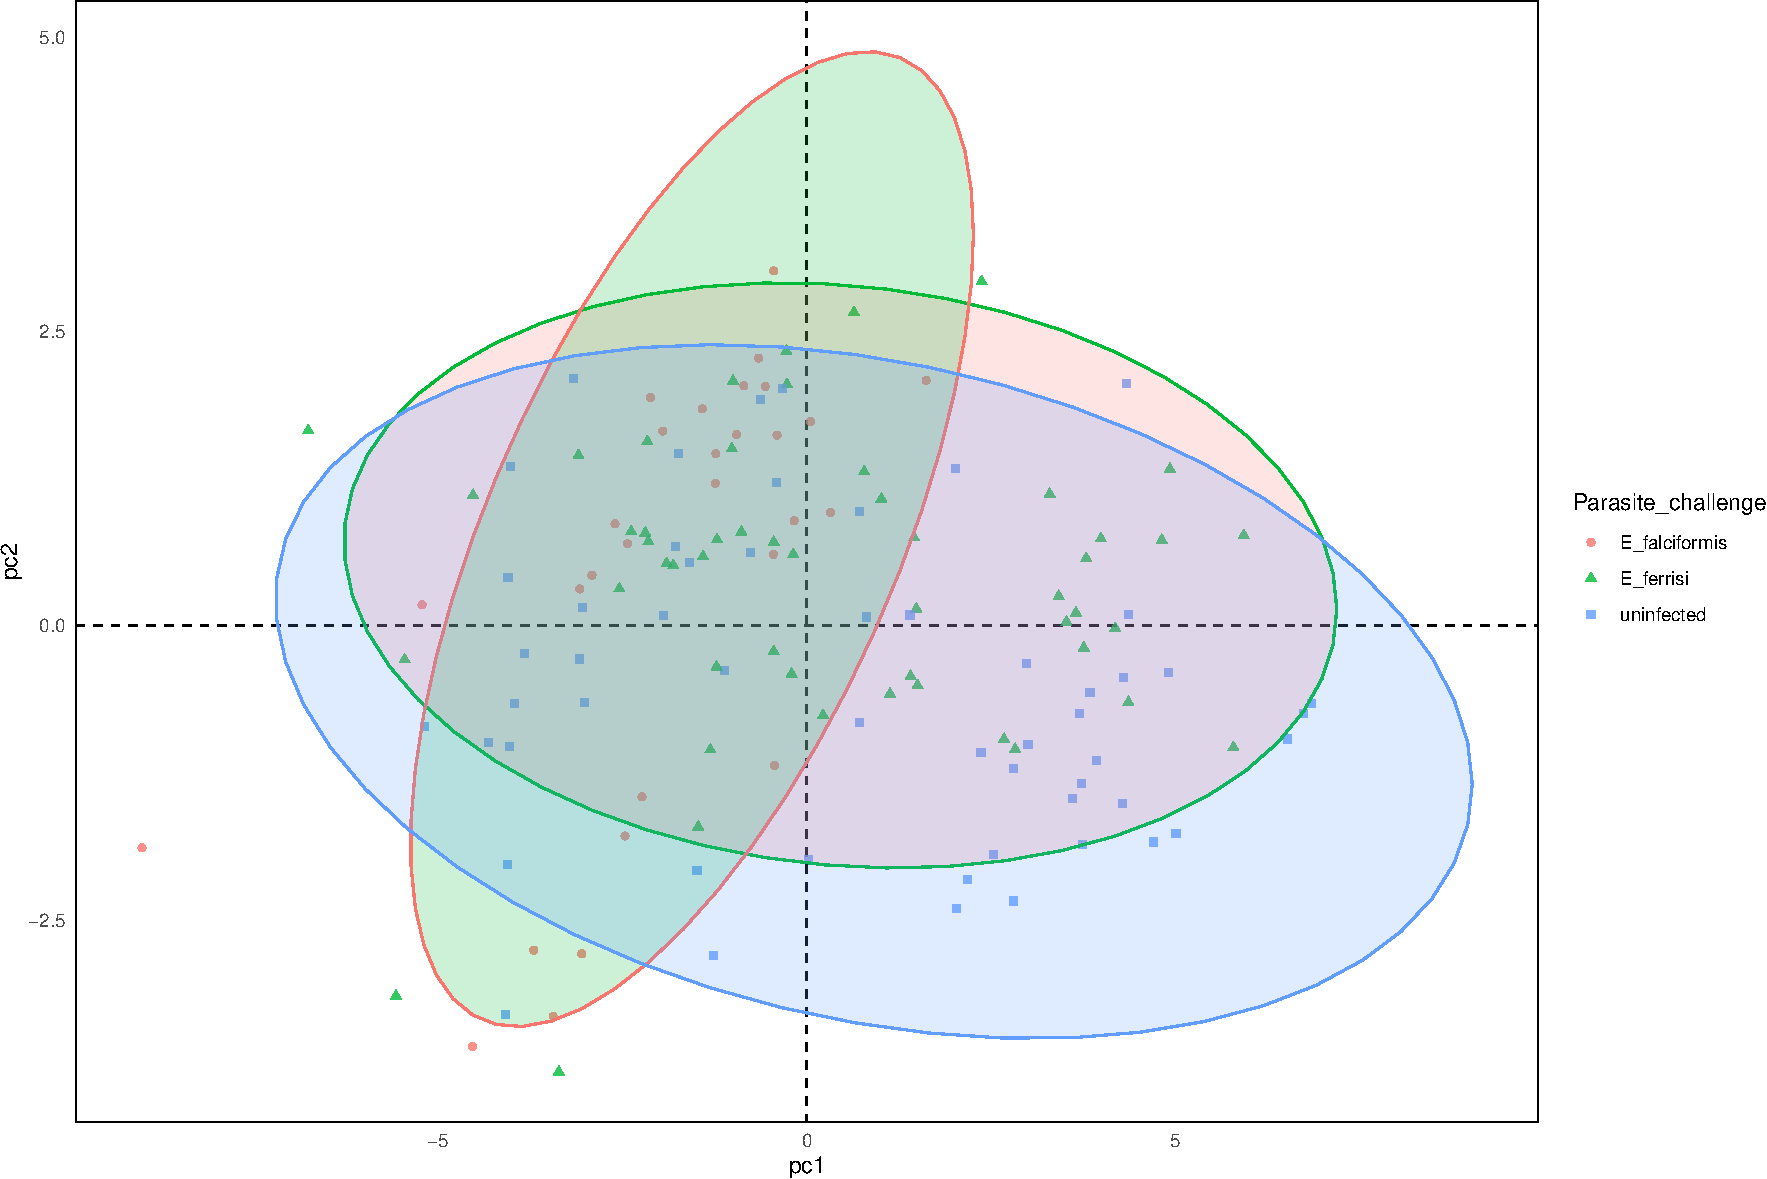
\includegraphics{1.Gene_expression_analysis_files/figure-latex/biplot_pca_genes-1.pdf}

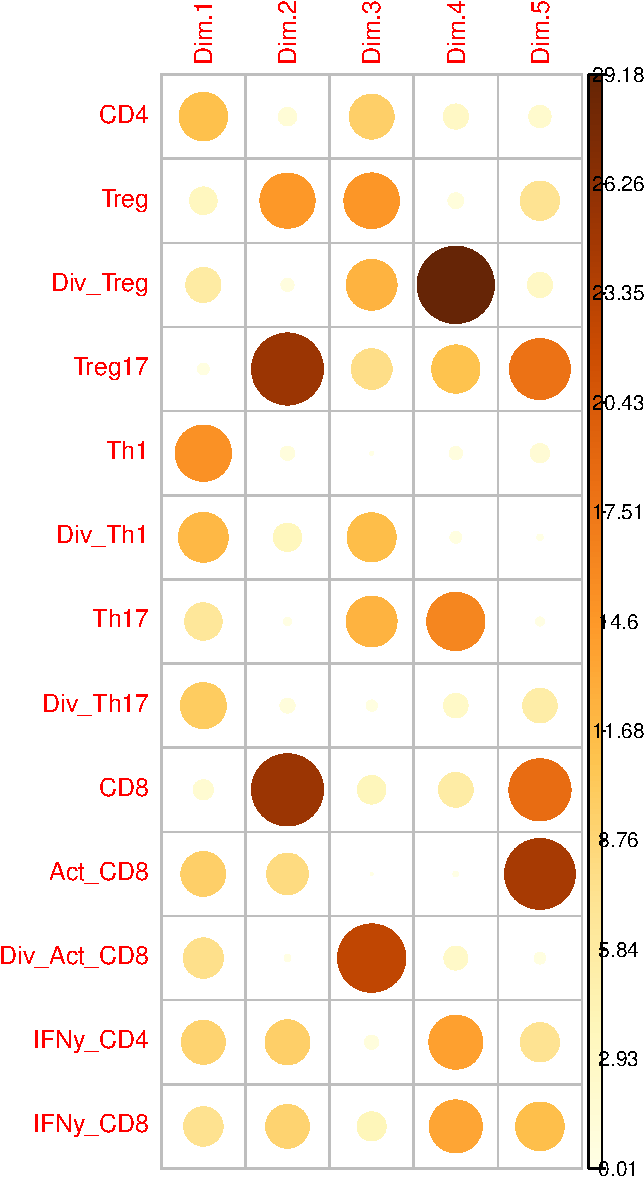
\includegraphics{1.Gene_expression_analysis_files/figure-latex/correlations_genes_dimensions-1.pdf}

The function fviz\_contrib() {[}factoextra package{]} can be used to
draw a bar plot of variable contributions. If your data contains many
variables, you can decide to show only the top contributing variables.
The R code below shows the top 10 variables contributing to the
principal components:

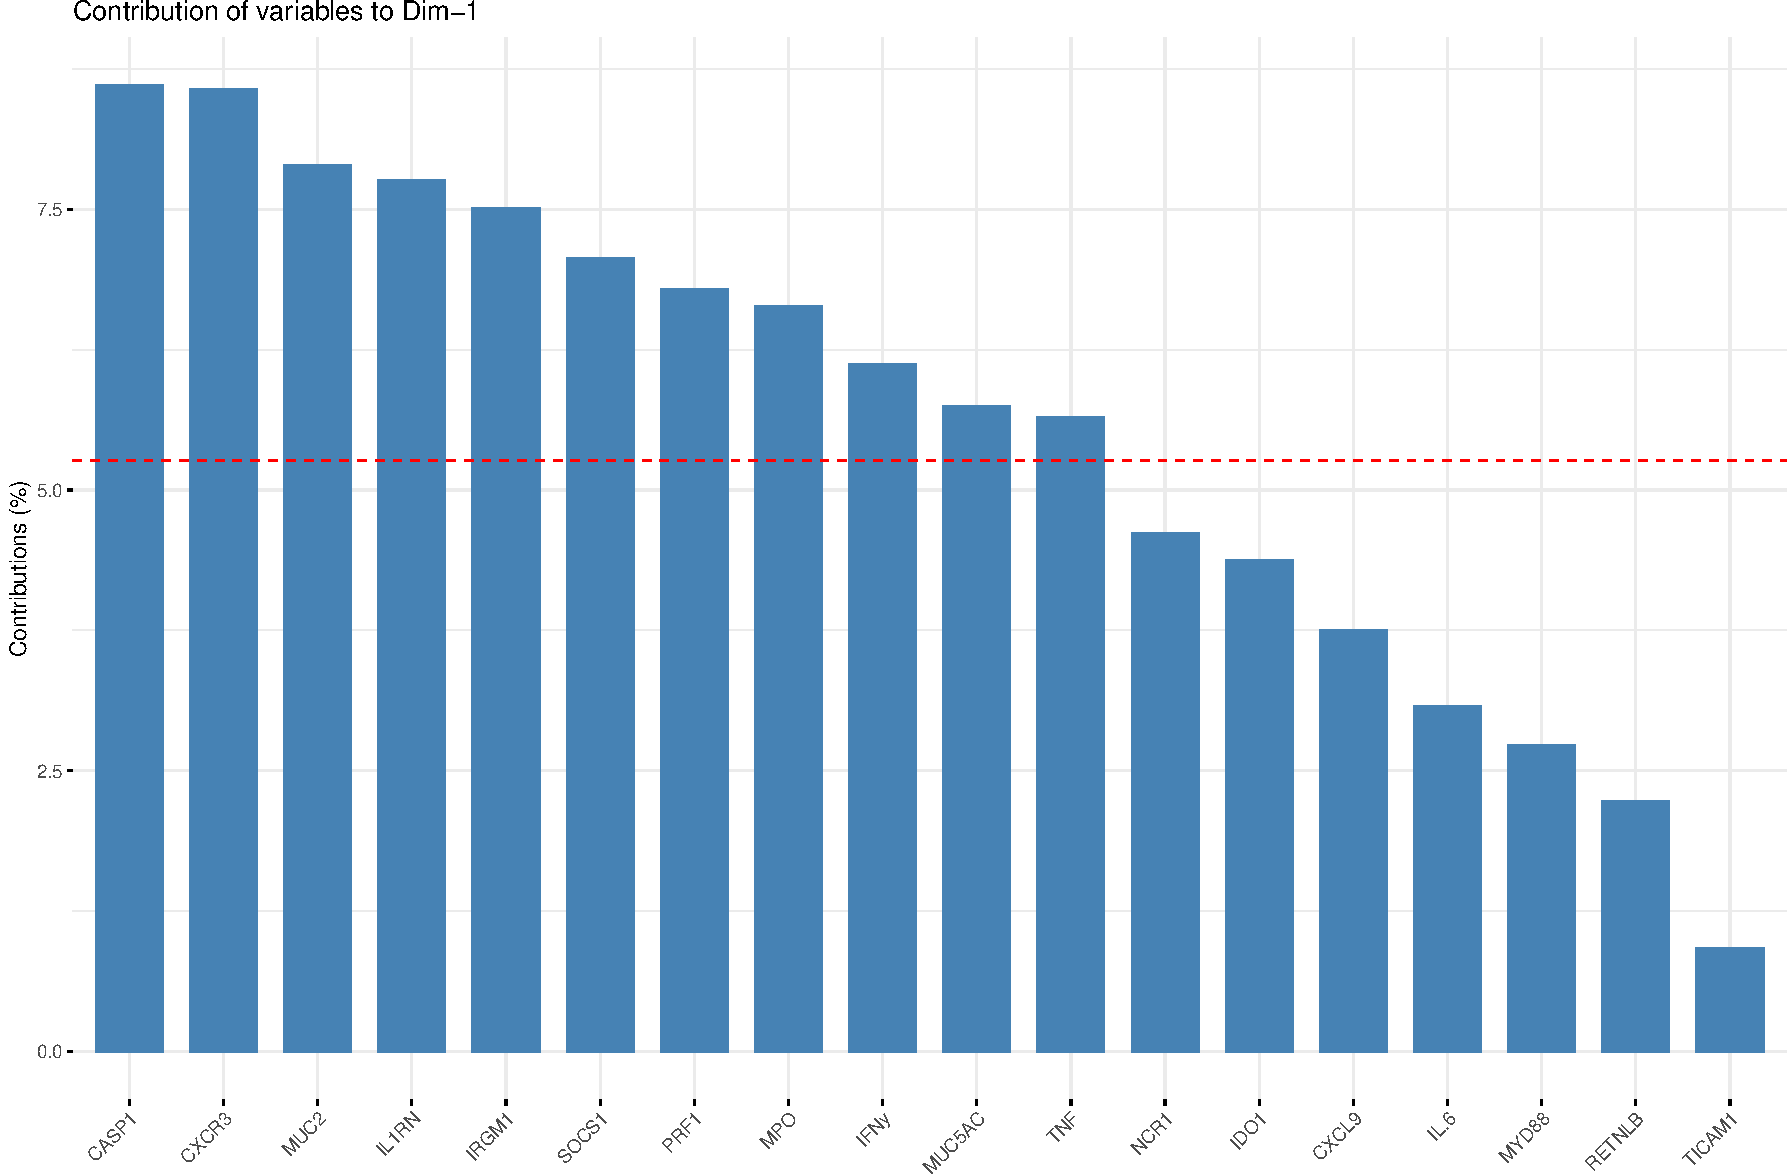
\includegraphics{1.Gene_expression_analysis_files/figure-latex/contr_var_pc_genes-1.pdf}

\begin{Shaded}
\begin{Highlighting}[]
\CommentTok{\# Contributions of variables to PC2}
\FunctionTok{fviz\_contrib}\NormalTok{(res.pca, }\AttributeTok{choice =} \StringTok{"var"}\NormalTok{, }\AttributeTok{axes =} \DecValTok{2}\NormalTok{, }\AttributeTok{top =} \DecValTok{18}\NormalTok{)}
\end{Highlighting}
\end{Shaded}

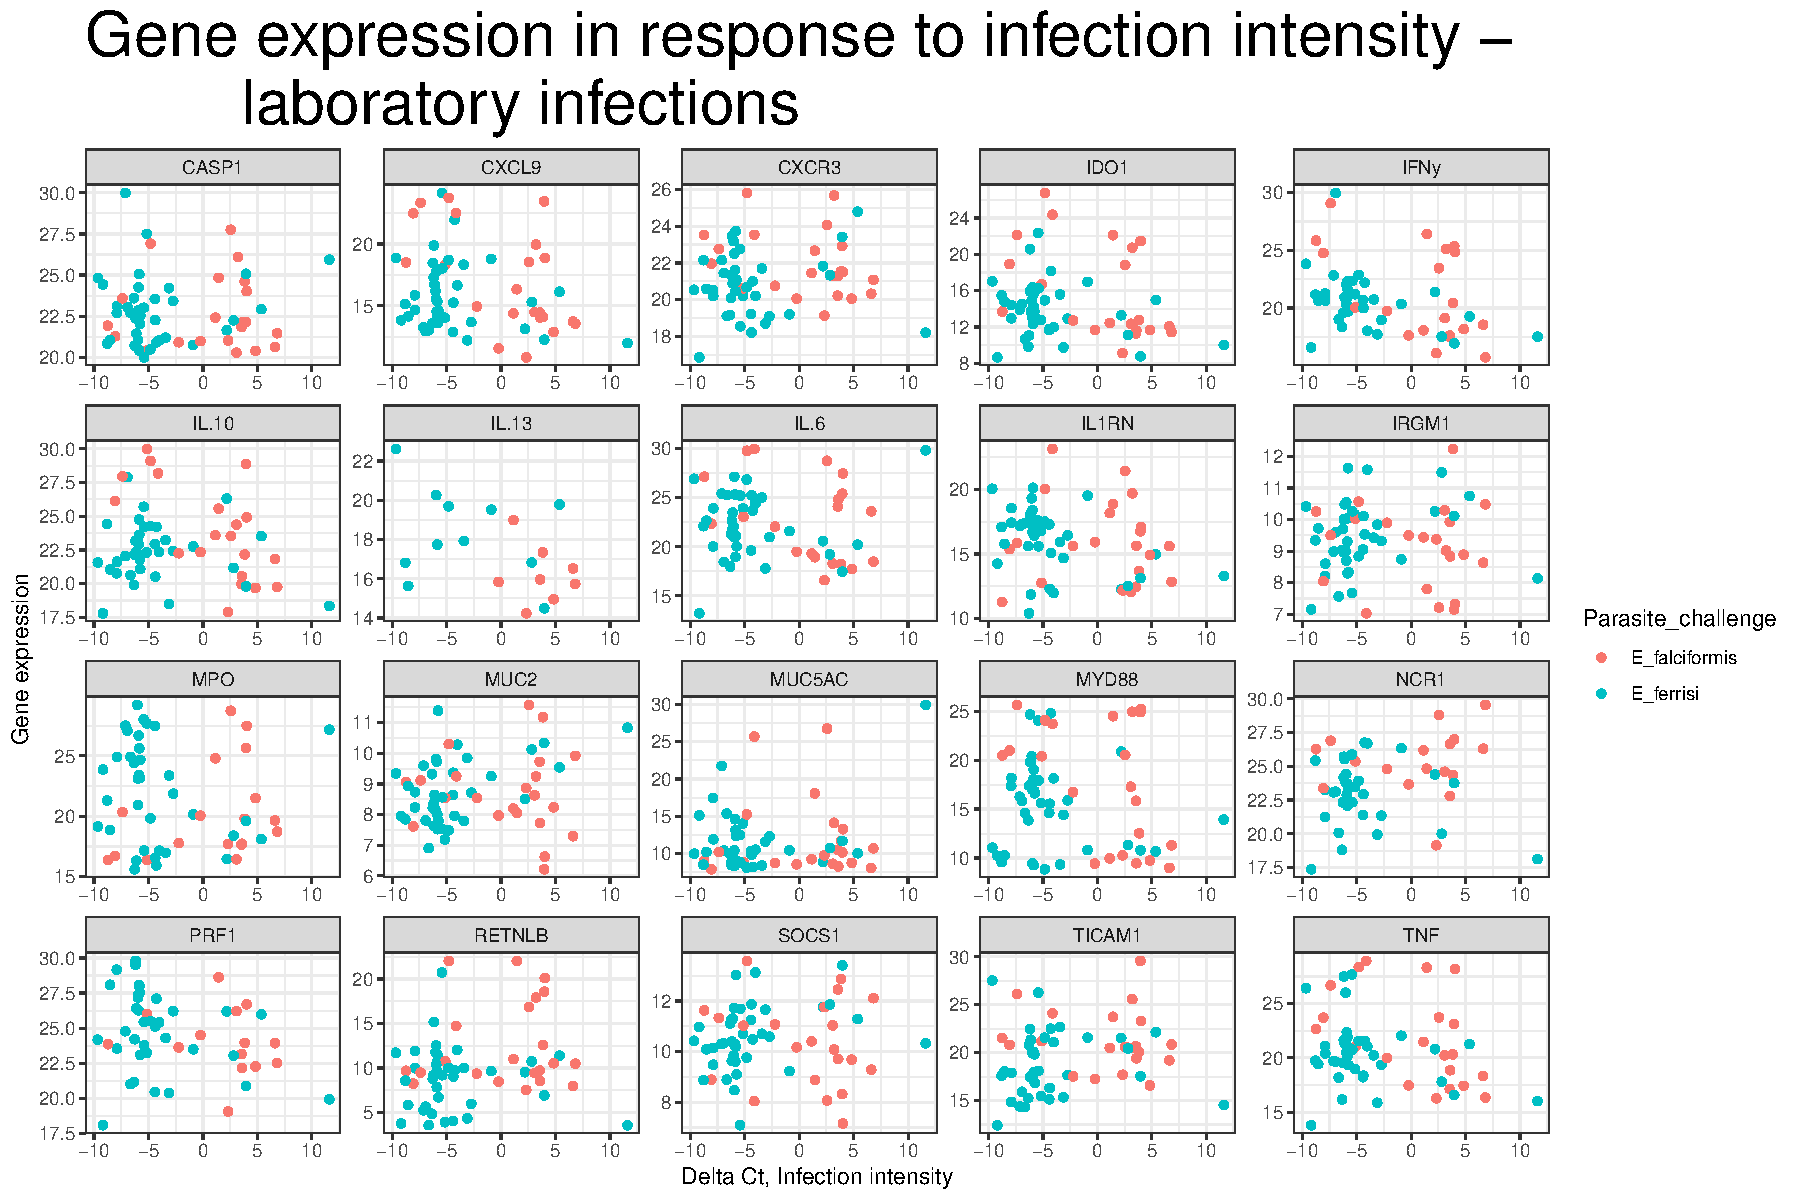
\includegraphics{1.Gene_expression_analysis_files/figure-latex/unnamed-chunk-4-1.pdf}

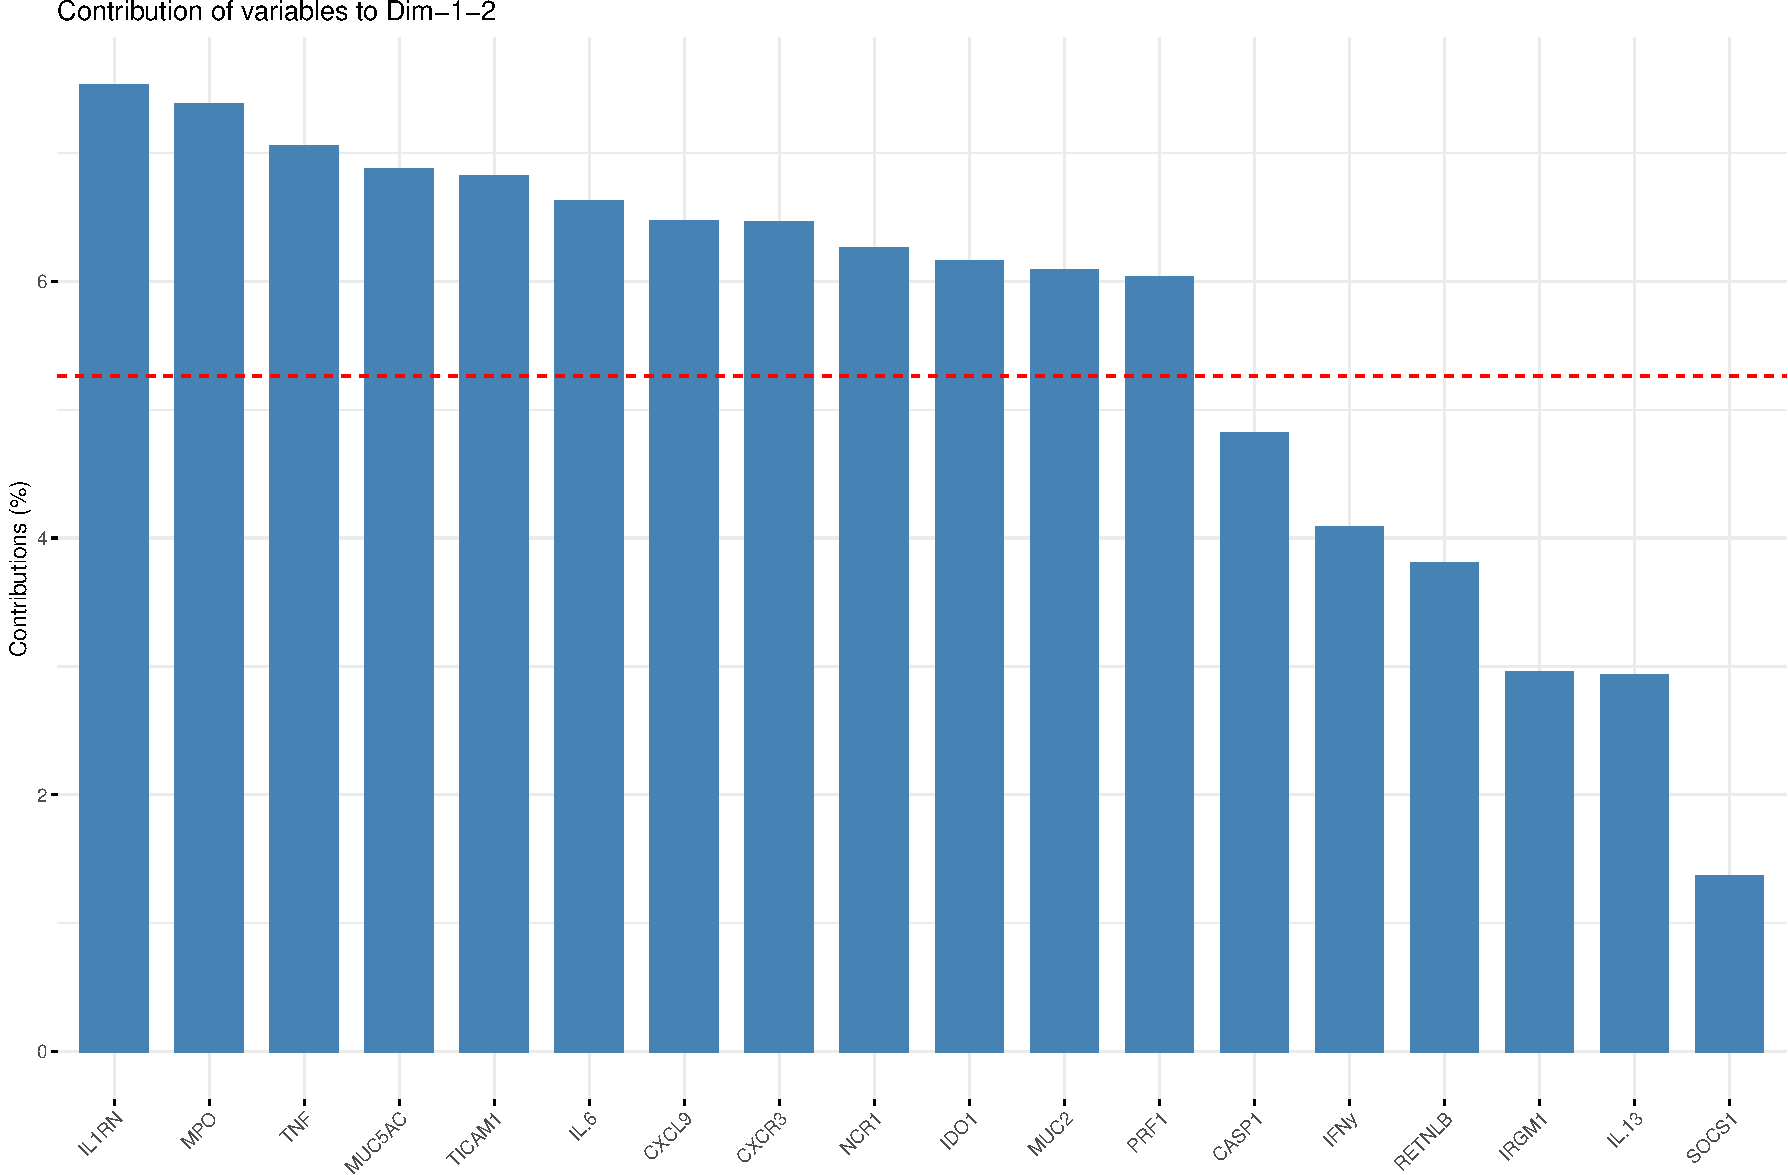
\includegraphics{1.Gene_expression_analysis_files/figure-latex/contr_var_pc1_2_genes-1.pdf}
The red dashed line on the graph above indicates the expected average
contribution. If the contribution of the variables were uniform, the
expected value would be 1/length(variables) = 1/10 = 10\%. For a given
component, a variable with a contribution larger than this cutoff could
be considered as important in contributing to the component.

Note that, the total contribution of a given variable, on explaining the
variations retained by two principal components, say PC1 and PC2, is
calculated as contrib = {[}(C1 * Eig1) + (C2 * Eig2){]}/(Eig1 + Eig2),
where

C1 and C2 are the contributions of the variable on PC1 and PC2,
respectively Eig1 and Eig2 are the eigenvalues of PC1 and PC2,
respectively. Recall that eigenvalues measure the amount of variation
retained by each PC. In this case, the expected average contribution
(cutoff) is calculated as follow: As mentioned above, if the
contributions of the 10 variables were uniform, the expected average
contribution on a given PC would be 1/10 = 10\%. The expected average
contribution of a variable for PC1 and PC2 is : {[}(10* Eig1) + (10 *
Eig2){]}/(Eig1 + Eig2)

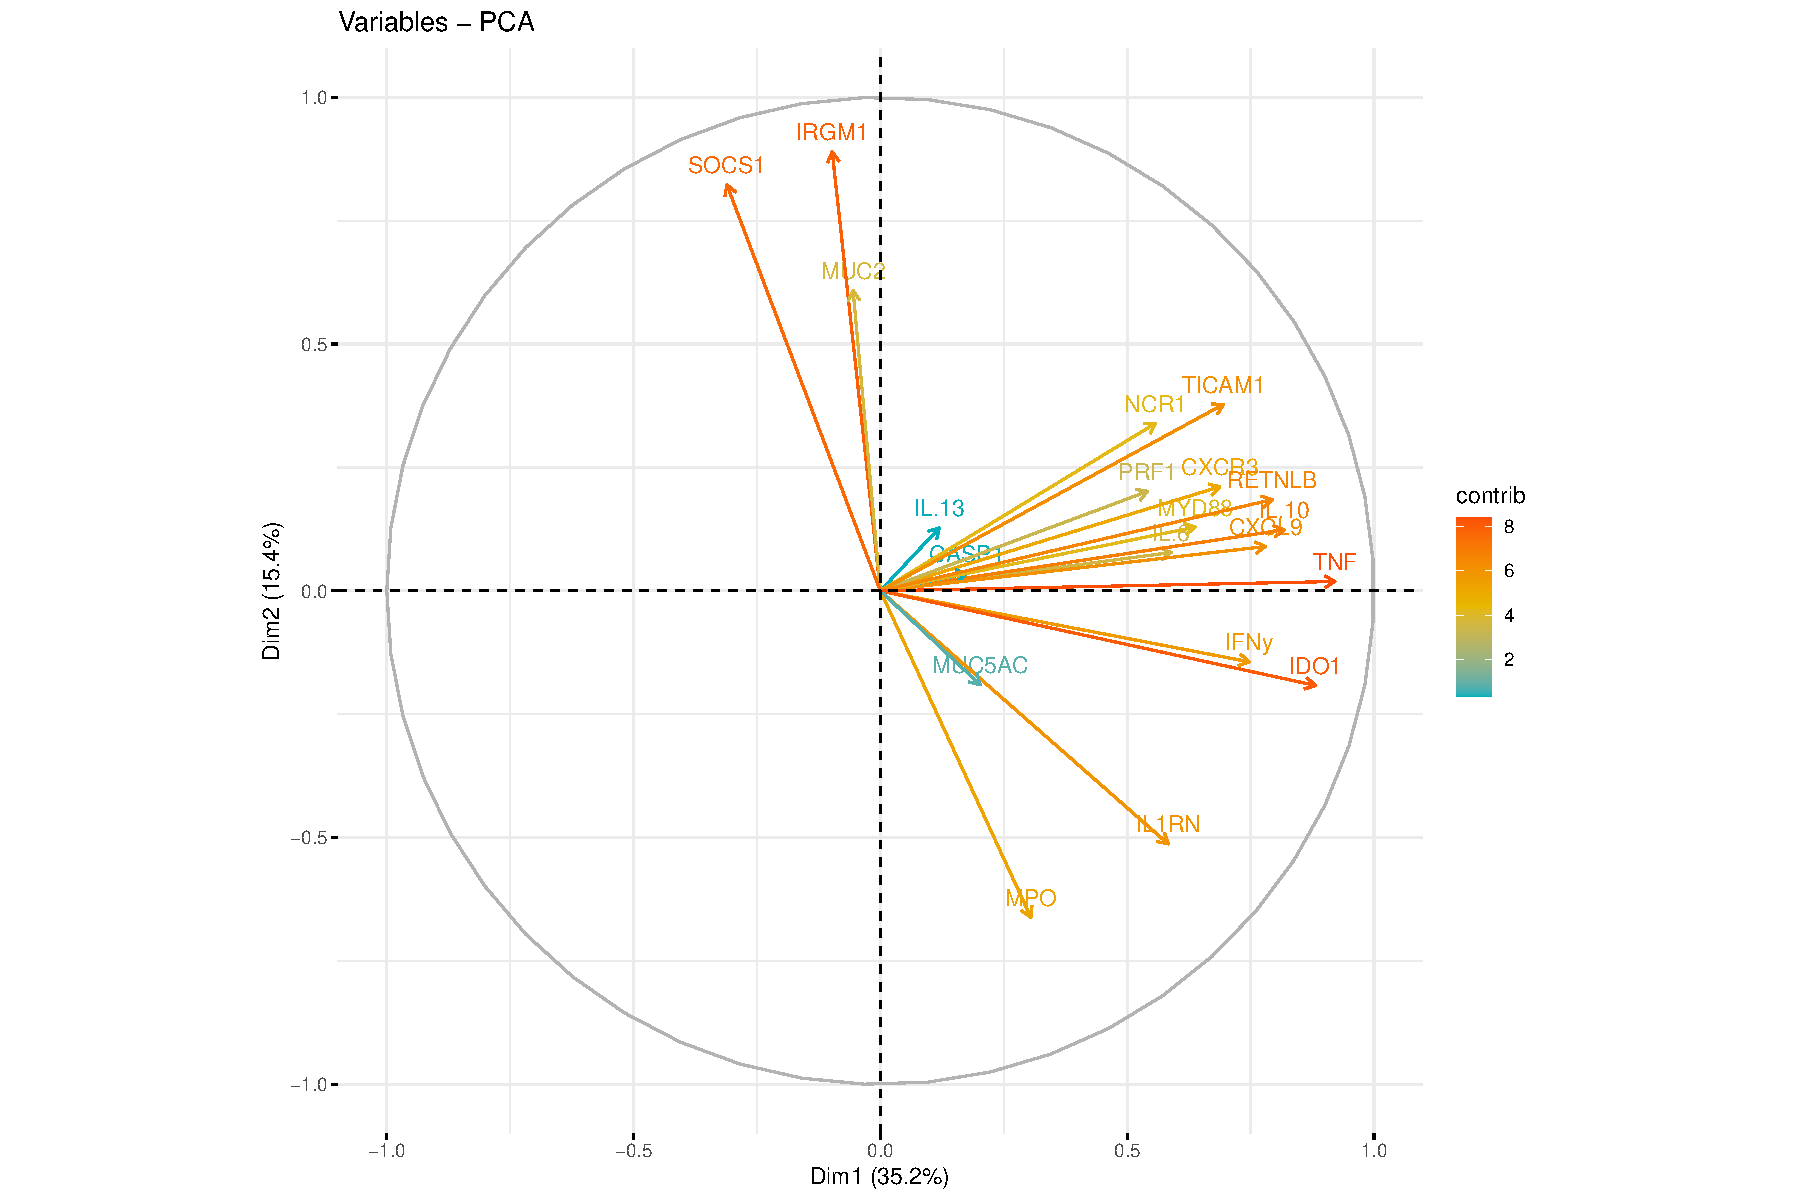
\includegraphics{1.Gene_expression_analysis_files/figure-latex/pca_contribution_genes-1.pdf}

To visualize the contribution of individuals to the first two principal
components:

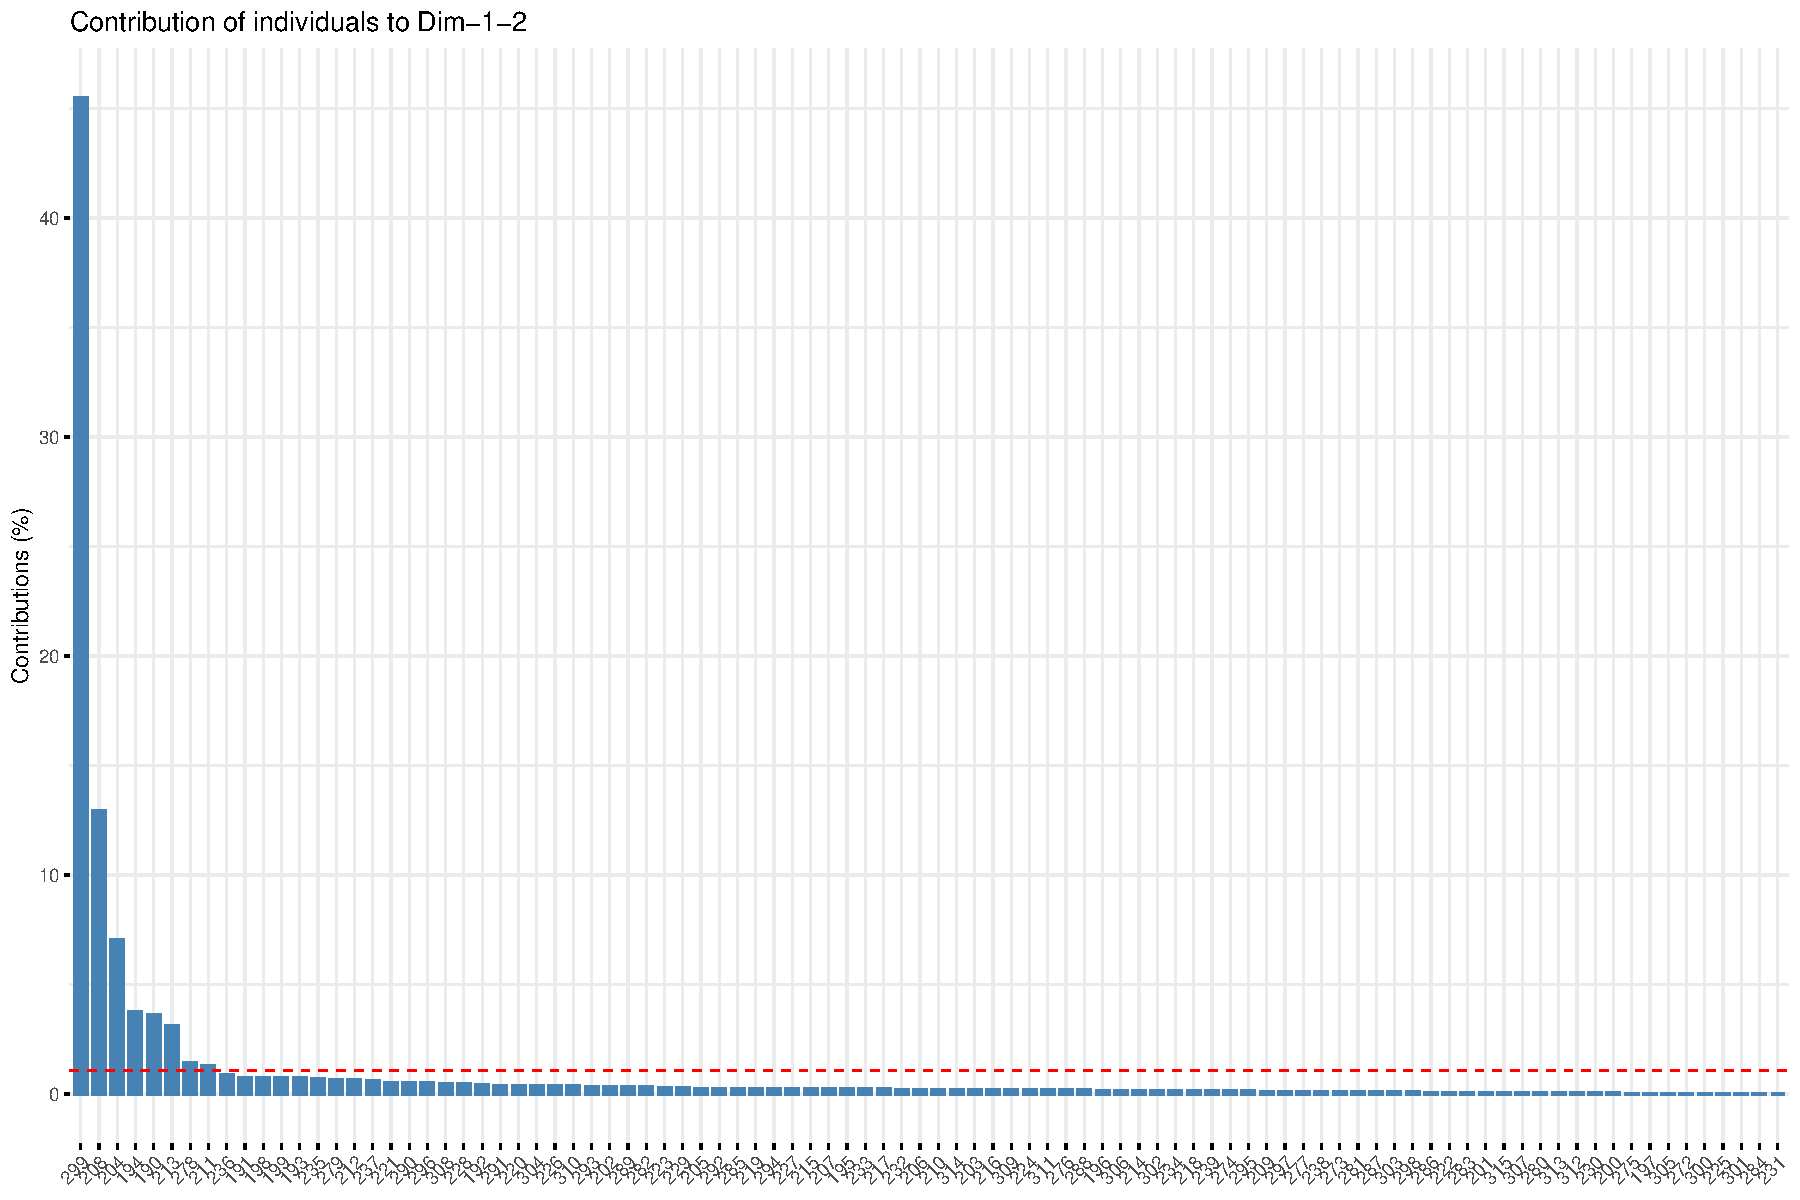
\includegraphics{1.Gene_expression_analysis_files/figure-latex/contr_individuals_genes-1.pdf}

PCA + Biplot combination

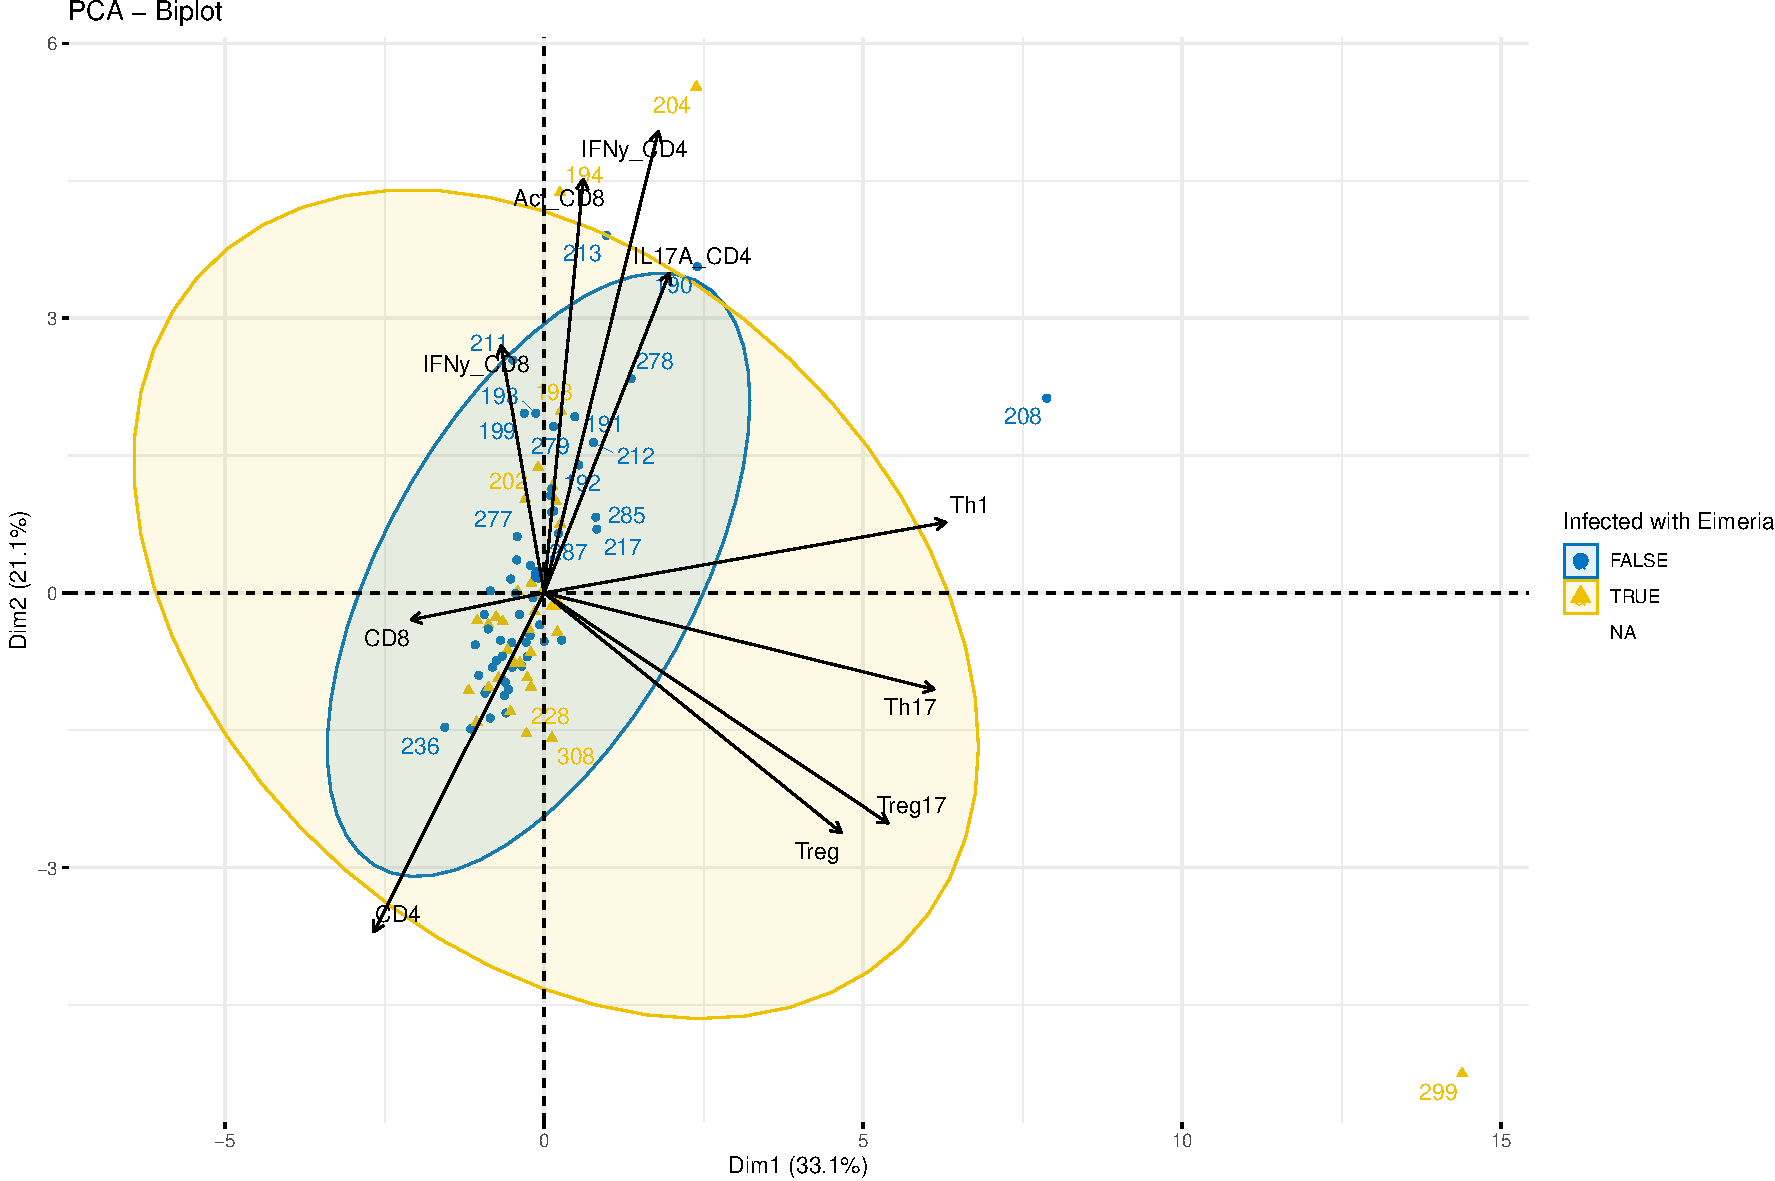
\includegraphics{1.Gene_expression_analysis_files/figure-latex/pca_biplot_genes-1.pdf}
In the following example, we want to color both individuals and
variables by groups. The trick is to use pointshape = 21 for individual
points. This particular point shape can be filled by a color using the
argument fill.ind. The border line color of individual points is set to
``black'' using col.ind. To color variable by groups, the argument
col.var will be used.

Linear models:

\begin{verbatim}
## 
## Call:
## lm(formula = max_WL ~ pc1 + pc2 + Parasite_challenge, data = imputed_expr)
## 
## Residuals:
##      Min       1Q   Median       3Q      Max 
## -14.2573  -3.0786   0.1754   3.5724  14.7045 
## 
## Coefficients:
##                              Estimate Std. Error t value Pr(>|t|)    
## (Intercept)                  85.25971    1.13926  74.838  < 2e-16 ***
## pc1                           0.08514    0.17453   0.488   0.6267    
## pc2                          -0.78042    0.28128  -2.775   0.0065 ** 
## Parasite_challengeE_ferrisi   6.43979    1.40275   4.591 1.18e-05 ***
## Parasite_challengeuninfected 10.91330    1.36065   8.021 1.23e-12 ***
## ---
## Signif. codes:  0 '***' 0.001 '**' 0.01 '*' 0.05 '.' 0.1 ' ' 1
## 
## Residual standard error: 5.182 on 110 degrees of freedom
## Multiple R-squared:  0.4029, Adjusted R-squared:  0.3812 
## F-statistic: 18.56 on 4 and 110 DF,  p-value: 1.113e-11
\end{verbatim}

\begin{verbatim}
## [1] 711.6453
\end{verbatim}

\begin{verbatim}
## 
## Call:
## lm(formula = max_WL ~ pc1 + pc2 + Parasite_challenge + hybrid_status, 
##     data = imputed_expr)
## 
## Residuals:
##      Min       1Q   Median       3Q      Max 
## -12.6298  -3.3747   0.6385   3.4840  14.2322 
## 
## Coefficients:
##                                  Estimate Std. Error t value Pr(>|t|)    
## (Intercept)                      85.75864    1.37658  62.298  < 2e-16 ***
## pc1                               0.09595    0.21657   0.443   0.6586    
## pc2                              -0.65606    0.31294  -2.096   0.0384 *  
## Parasite_challengeE_ferrisi       6.25599    1.44754   4.322 3.53e-05 ***
## Parasite_challengeuninfected     10.52958    1.45328   7.245 7.53e-11 ***
## hybrid_statusF0 M. m. musculus   -1.27996    1.44023  -0.889   0.3762    
## hybrid_statusF1 hybrid            1.24135    1.66604   0.745   0.4579    
## hybrid_statusF1 M. m. domesticus -1.91599    2.18568  -0.877   0.3827    
## hybrid_statusF1 M. m. musculus    1.45554    2.65578   0.548   0.5848    
## hybrid_statusother               -0.54848    1.46912  -0.373   0.7096    
## ---
## Signif. codes:  0 '***' 0.001 '**' 0.01 '*' 0.05 '.' 0.1 ' ' 1
## 
## Residual standard error: 5.221 on 105 degrees of freedom
## Multiple R-squared:  0.4215, Adjusted R-squared:  0.3719 
## F-statistic: 8.501 on 9 and 105 DF,  p-value: 1.841e-09
\end{verbatim}

\begin{verbatim}
## [1] 718.0054
\end{verbatim}

Try instead: LLR test (likelihood ration) (LM4 package )?

\url{https://www.rdocumentation.org/packages/lmtest/versions/0.9-38/topics/lrtest}

In this way you compare each model, with the different variables usesd
to predict.

Another way is to compare the AIC. (function : step)

\begin{Shaded}
\begin{Highlighting}[]
\NormalTok{weight\_lm3 }\OtherTok{\textless{}{-}} \FunctionTok{lm}\NormalTok{(max\_WL }\SpecialCharTok{\textasciitilde{}}\NormalTok{ pc1 }\SpecialCharTok{+}\NormalTok{ pc2 }\SpecialCharTok{+}\NormalTok{ hybrid\_status, }\AttributeTok{data =}\NormalTok{ imputed\_expr)}
\NormalTok{weight\_no\_pc1 }\OtherTok{\textless{}{-}} \FunctionTok{lm}\NormalTok{(max\_WL }\SpecialCharTok{\textasciitilde{}}\NormalTok{ pc2 }\SpecialCharTok{+}\NormalTok{ hybrid\_status, }\AttributeTok{data =}\NormalTok{ imputed\_expr)}
\NormalTok{weight\_no\_pc2 }\OtherTok{\textless{}{-}} \FunctionTok{lm}\NormalTok{(max\_WL }\SpecialCharTok{\textasciitilde{}}\NormalTok{ pc1  }\SpecialCharTok{+}\NormalTok{ hybrid\_status, }\AttributeTok{data =}\NormalTok{ imputed\_expr)}
\NormalTok{weight\_no\_hybrid }\OtherTok{\textless{}{-}} \FunctionTok{lm}\NormalTok{(max\_WL }\SpecialCharTok{\textasciitilde{}}\NormalTok{ pc1 }\SpecialCharTok{+}\NormalTok{ pc2, }\AttributeTok{data =}\NormalTok{ imputed\_expr)}
\FunctionTok{lrtest}\NormalTok{(weight\_lm3, weight\_no\_pc1)}
\end{Highlighting}
\end{Shaded}

\begin{verbatim}
## Likelihood ratio test
## 
## Model 1: max_WL ~ pc1 + pc2 + hybrid_status
## Model 2: max_WL ~ pc2 + hybrid_status
##   #Df  LogLik Df Chisq Pr(>Chisq)
## 1   9 -371.59                    
## 2   8 -372.82 -1  2.46     0.1168
\end{verbatim}

\begin{Shaded}
\begin{Highlighting}[]
\FunctionTok{lrtest}\NormalTok{(weight\_lm3, weight\_no\_pc2)}
\end{Highlighting}
\end{Shaded}

\begin{verbatim}
## Likelihood ratio test
## 
## Model 1: max_WL ~ pc1 + pc2 + hybrid_status
## Model 2: max_WL ~ pc1 + hybrid_status
##   #Df  LogLik Df  Chisq Pr(>Chisq)
## 1   9 -371.59                     
## 2   8 -372.06 -1 0.9509     0.3295
\end{verbatim}

\begin{Shaded}
\begin{Highlighting}[]
\FunctionTok{lrtest}\NormalTok{(weight\_lm3, weight\_no\_hybrid)}
\end{Highlighting}
\end{Shaded}

\begin{verbatim}
## Likelihood ratio test
## 
## Model 1: max_WL ~ pc1 + pc2 + hybrid_status
## Model 2: max_WL ~ pc1 + pc2
##   #Df  LogLik Df  Chisq Pr(>Chisq)  
## 1   9 -371.59                       
## 2   4 -376.66 -5 10.136    0.07147 .
## ---
## Signif. codes:  0 '***' 0.001 '**' 0.01 '*' 0.05 '.' 0.1 ' ' 1
\end{verbatim}

\begin{verbatim}
## 
## Call:
## lm(formula = max_WL ~ pc1 + pc2 + hybrid_status, data = imputed_expr)
## 
## Residuals:
##      Min       1Q   Median       3Q      Max 
## -15.9569  -3.1589   0.9603   4.7902   9.9729 
## 
## Coefficients:
##                                  Estimate Std. Error t value Pr(>|t|)    
## (Intercept)                       92.5224     1.0361  89.298   <2e-16 ***
## pc1                                0.3795     0.2495   1.521   0.1312    
## pc2                               -0.3522     0.3737  -0.943   0.3480    
## hybrid_statusF0 M. m. musculus    -1.1797     1.7494  -0.674   0.5015    
## hybrid_statusF1 hybrid             3.6953     1.9838   1.863   0.0652 .  
## hybrid_statusF1 M. m. domesticus  -0.3532     2.6390  -0.134   0.8938    
## hybrid_statusF1 M. m. musculus     3.8882     3.2042   1.213   0.2276    
## hybrid_statusother                -2.6956     1.7504  -1.540   0.1265    
## ---
## Signif. codes:  0 '***' 0.001 '**' 0.01 '*' 0.05 '.' 0.1 ' ' 1
## 
## Residual standard error: 6.349 on 107 degrees of freedom
## Multiple R-squared:  0.1282, Adjusted R-squared:  0.07114 
## F-statistic: 2.247 on 7 and 107 DF,  p-value: 0.03582
\end{verbatim}

\begin{verbatim}
## [1] 761.1772
\end{verbatim}

\begin{verbatim}
## 
## Call:
## lm(formula = max_WL ~ pc1 + pc2 + infection_history, data = imputed_expr)
## 
## Residuals:
##      Min       1Q   Median       3Q      Max 
## -13.4092  -3.5729   0.2862   2.9779  14.3702 
## 
## Coefficients:
##                                          Estimate Std. Error t value Pr(>|t|)
## (Intercept)                             89.135470   2.083975  42.772  < 2e-16
## pc1                                      0.009692   0.172513   0.056  0.95530
## pc2                                     -0.636620   0.294681  -2.160  0.03304
## infection_historyfalciformis_ferrisi     3.012046   2.440778   1.234  0.21997
## infection_historyfalciformis_uninfected  7.691011   2.474342   3.108  0.00243
## infection_historyferrisi_falciformis    -6.631688   2.665453  -2.488  0.01443
## infection_historyferrisi_ferrisi         3.680451   2.425754   1.517  0.13224
## infection_historyferrisi_uninfected      6.371904   2.303272   2.766  0.00671
## infection_historyuninfected              8.164906   2.713643   3.009  0.00329
## infection_historyuninfected_falciformis -3.586390   2.916467  -1.230  0.22158
## infection_historyuninfected_ferrisi     -1.672385   2.758361  -0.606  0.54564
##                                            
## (Intercept)                             ***
## pc1                                        
## pc2                                     *  
## infection_historyfalciformis_ferrisi       
## infection_historyfalciformis_uninfected ** 
## infection_historyferrisi_falciformis    *  
## infection_historyferrisi_ferrisi           
## infection_historyferrisi_uninfected     ** 
## infection_historyuninfected             ** 
## infection_historyuninfected_falciformis    
## infection_historyuninfected_ferrisi        
## ---
## Signif. codes:  0 '***' 0.001 '**' 0.01 '*' 0.05 '.' 0.1 ' ' 1
## 
## Residual standard error: 5.006 on 104 degrees of freedom
## Multiple R-squared:  0.4732, Adjusted R-squared:  0.4226 
## F-statistic: 9.343 on 10 and 104 DF,  p-value: 6.704e-11
\end{verbatim}

\begin{verbatim}
## [1] 709.2351
\end{verbatim}

\begin{verbatim}
## 
## Call:
## lm(formula = max_WL ~ pc1 + pc2, data = imputed_expr)
## 
## Residuals:
##     Min      1Q  Median      3Q     Max 
## -16.884  -3.286   1.368   5.175  10.615 
## 
## Coefficients:
##             Estimate Std. Error t value Pr(>|t|)    
## (Intercept)  92.3518     0.6048 152.707   <2e-16 ***
## pc1           0.1624     0.2080   0.781    0.437    
## pc2          -0.7795     0.3480  -2.240    0.027 *  
## ---
## Signif. codes:  0 '***' 0.001 '**' 0.01 '*' 0.05 '.' 0.1 ' ' 1
## 
## Residual standard error: 6.485 on 112 degrees of freedom
## Multiple R-squared:  0.04785,    Adjusted R-squared:  0.03084 
## F-statistic: 2.814 on 2 and 112 DF,  p-value: 0.0642
\end{verbatim}

\begin{verbatim}
##                    df      AIC
## weight_lm           6 711.6453
## weight_lm_exp_only  4 761.3132
\end{verbatim}

\hypertarget{repeating-the-heatmap-on-the-now-imputed-data}{%
\subsubsection{repeating the heatmap on the now imputed
data}\label{repeating-the-heatmap-on-the-now-imputed-data}}

\begin{Shaded}
\begin{Highlighting}[]
\NormalTok{gene }\OtherTok{\textless{}{-}}\NormalTok{ imputed\_expr }\SpecialCharTok{\%\textgreater{}\%}\NormalTok{ dplyr}\SpecialCharTok{::}\FunctionTok{select}\NormalTok{(}\FunctionTok{c}\NormalTok{(EH\_ID, }\FunctionTok{all\_of}\NormalTok{(Genes)))}
 
 \CommentTok{\# turn the data frame into a matrix and transpose it. We want to have each cell }
 \CommentTok{\# type as a row name }
\NormalTok{ gene }\OtherTok{\textless{}{-}} \FunctionTok{t}\NormalTok{(}\FunctionTok{as.matrix}\NormalTok{(gene))}
 
 \CommentTok{\#switch the matrix back to a data frame format}
\NormalTok{ gene }\OtherTok{\textless{}{-}} \FunctionTok{as.data.frame}\NormalTok{(gene)}
 
 \CommentTok{\# turn the first row into column names}
\NormalTok{ gene }\SpecialCharTok{\%\textgreater{}\%}
     \FunctionTok{row\_to\_names}\NormalTok{(}\AttributeTok{row\_number =} \DecValTok{1}\NormalTok{) }\OtherTok{{-}\textgreater{}}\NormalTok{ heatmap\_data}
 
 
 \FunctionTok{table}\NormalTok{(}\FunctionTok{rowSums}\NormalTok{(}\FunctionTok{is.na}\NormalTok{(heatmap\_data)) }\SpecialCharTok{==} \FunctionTok{nrow}\NormalTok{(heatmap\_data))}
\end{Highlighting}
\end{Shaded}

\begin{verbatim}
## 
## FALSE 
##    20
\end{verbatim}

\begin{Shaded}
\begin{Highlighting}[]
 \CommentTok{\# turn the columns to numeric other wise the heatmap function will not work}
\NormalTok{ heatmap\_data[] }\OtherTok{\textless{}{-}} \FunctionTok{lapply}\NormalTok{(heatmap\_data, }\ControlFlowTok{function}\NormalTok{(x) }\FunctionTok{as.numeric}\NormalTok{(}\FunctionTok{as.character}\NormalTok{(x)))}

 \CommentTok{\# remove columns with only NAs }
\NormalTok{ heatmap\_data }\OtherTok{\textless{}{-}} \FunctionTok{Filter}\NormalTok{(}\ControlFlowTok{function}\NormalTok{(x)}\SpecialCharTok{!}\FunctionTok{all}\NormalTok{(}\FunctionTok{is.na}\NormalTok{(x)), heatmap\_data) }
 
 \CommentTok{\#remove rows with only Nas}
\NormalTok{ heatmap\_data }\OtherTok{\textless{}{-}}\NormalTok{  heatmap\_data[, }\FunctionTok{colSums}\NormalTok{(}\FunctionTok{is.na}\NormalTok{(heatmap\_data)) }\SpecialCharTok{!=} \FunctionTok{nrow}\NormalTok{(heatmap\_data)]}

\FunctionTok{rownames}\NormalTok{(annotation\_df) }\OtherTok{\textless{}{-}} \FunctionTok{colnames}\NormalTok{(heatmap\_data)}
\end{Highlighting}
\end{Shaded}

Heatmap on gene expression data:

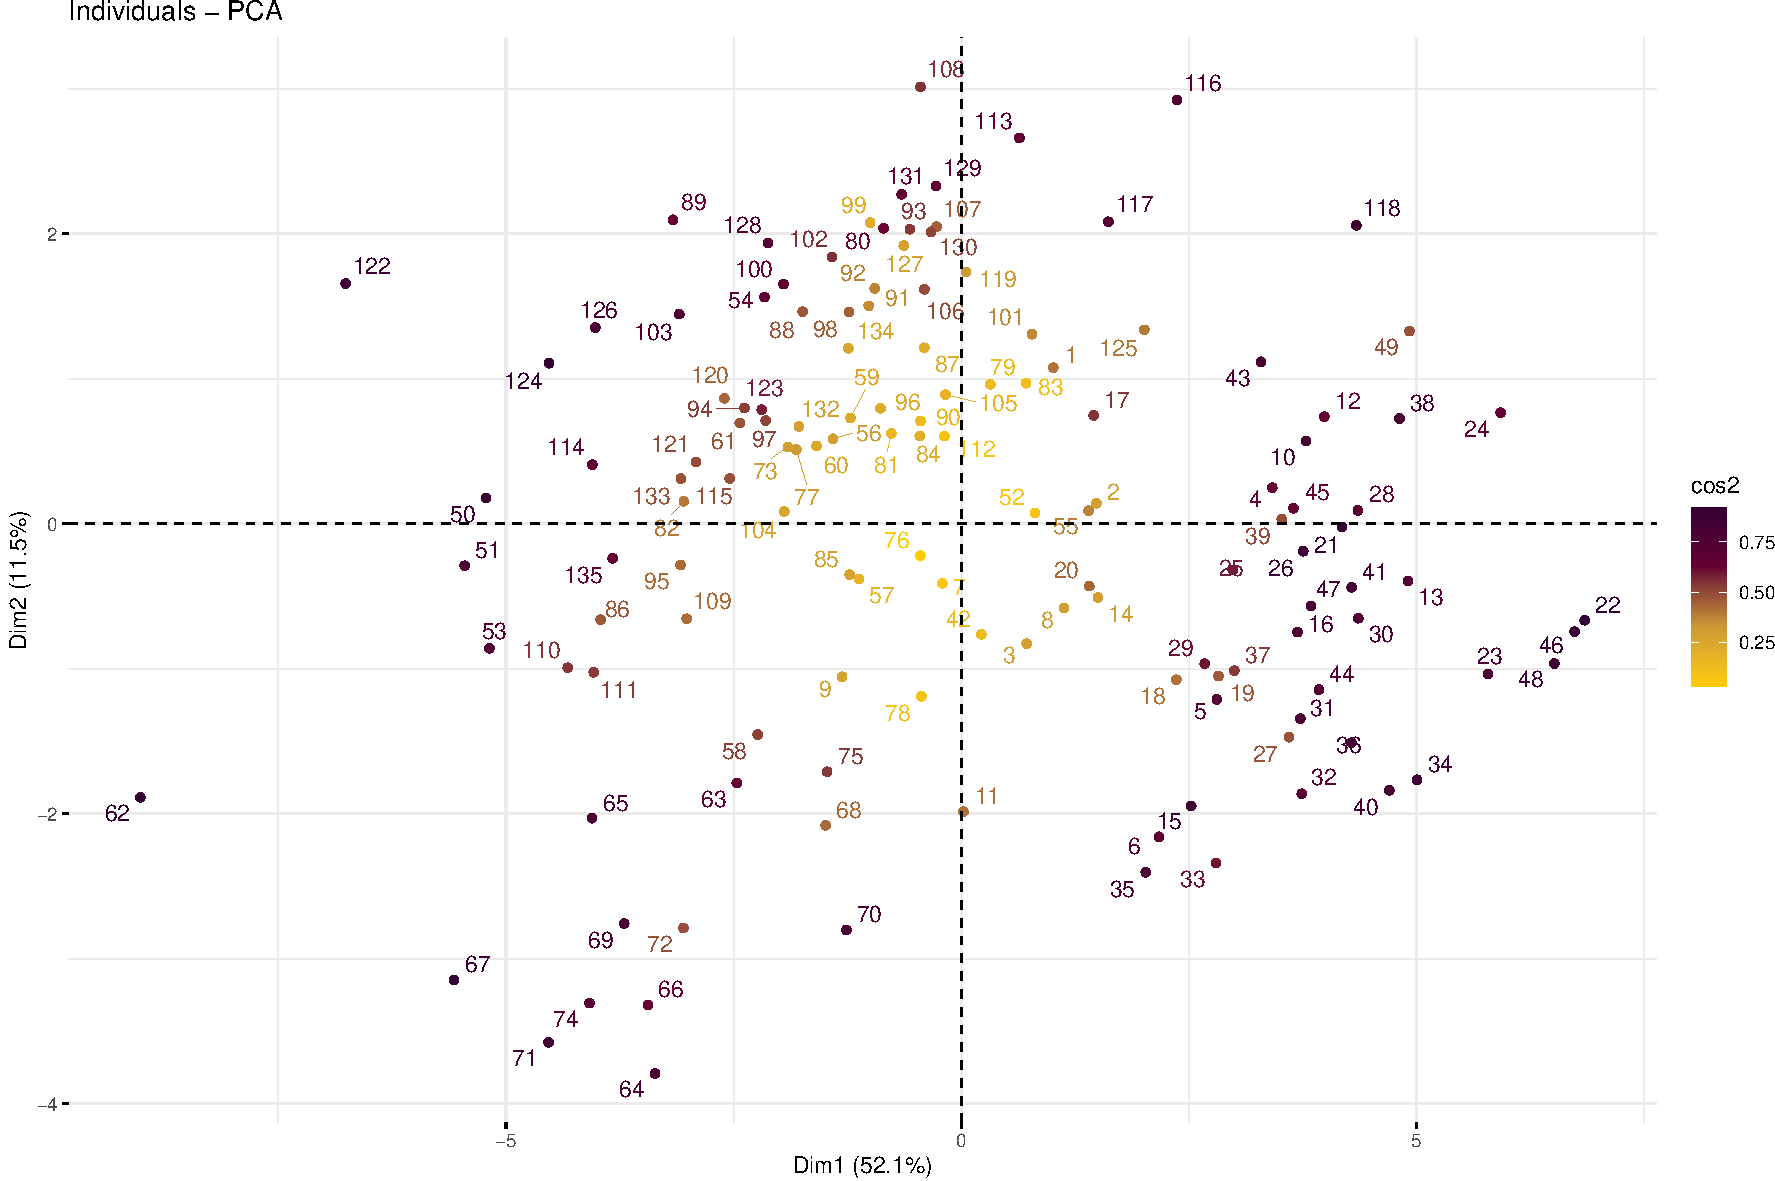
\includegraphics{1.Gene_expression_analysis_files/figure-latex/unnamed-chunk-7-1.pdf}

\hypertarget{repeating-the-heatmap-on-the-significant-genes-imputed-data}{%
\subsubsection{repeating the heatmap on the significant genes imputed
data}\label{repeating-the-heatmap-on-the-significant-genes-imputed-data}}

\begin{Shaded}
\begin{Highlighting}[]
\NormalTok{gene }\OtherTok{\textless{}{-}}\NormalTok{ imputed\_expr }\SpecialCharTok{\%\textgreater{}\%}\NormalTok{ dplyr}\SpecialCharTok{::}\FunctionTok{select}\NormalTok{(}\FunctionTok{c}\NormalTok{(EH\_ID, }\FunctionTok{c}\NormalTok{(}\StringTok{"IFNy"}\NormalTok{, }\StringTok{"IL.13"}\NormalTok{, }\StringTok{"PRF1"}\NormalTok{, }
                                                  \StringTok{"TICAM1"}\NormalTok{)))}
 
 \CommentTok{\# turn the data frame into a matrix and transpose it. We want to have each cell }
 \CommentTok{\# type as a row name }
\NormalTok{ gene }\OtherTok{\textless{}{-}} \FunctionTok{t}\NormalTok{(}\FunctionTok{as.matrix}\NormalTok{(gene))}
 
 \CommentTok{\#switch the matrix back to a data frame format}
\NormalTok{ gene }\OtherTok{\textless{}{-}} \FunctionTok{as.data.frame}\NormalTok{(gene)}
 
 \CommentTok{\# turn the first row into column names}
\NormalTok{ gene }\SpecialCharTok{\%\textgreater{}\%}
     \FunctionTok{row\_to\_names}\NormalTok{(}\AttributeTok{row\_number =} \DecValTok{1}\NormalTok{) }\OtherTok{{-}\textgreater{}}\NormalTok{ heatmap\_data}
 
 
 \FunctionTok{table}\NormalTok{(}\FunctionTok{rowSums}\NormalTok{(}\FunctionTok{is.na}\NormalTok{(heatmap\_data)) }\SpecialCharTok{==} \FunctionTok{nrow}\NormalTok{(heatmap\_data))}
\end{Highlighting}
\end{Shaded}

\begin{verbatim}
## 
## FALSE 
##     4
\end{verbatim}

\begin{Shaded}
\begin{Highlighting}[]
 \CommentTok{\# turn the columns to numeric other wise the heatmap function will not work}
\NormalTok{ heatmap\_data[] }\OtherTok{\textless{}{-}} \FunctionTok{lapply}\NormalTok{(heatmap\_data, }\ControlFlowTok{function}\NormalTok{(x) }\FunctionTok{as.numeric}\NormalTok{(}\FunctionTok{as.character}\NormalTok{(x)))}

 \CommentTok{\# remove columns with only NAs }
\NormalTok{ heatmap\_data }\OtherTok{\textless{}{-}} \FunctionTok{Filter}\NormalTok{(}\ControlFlowTok{function}\NormalTok{(x)}\SpecialCharTok{!}\FunctionTok{all}\NormalTok{(}\FunctionTok{is.na}\NormalTok{(x)), heatmap\_data) }
 
 \CommentTok{\#remove rows with only Nas}
\NormalTok{ heatmap\_data }\OtherTok{\textless{}{-}}\NormalTok{  heatmap\_data[, }\FunctionTok{colSums}\NormalTok{(}\FunctionTok{is.na}\NormalTok{(heatmap\_data)) }\SpecialCharTok{!=} \FunctionTok{nrow}\NormalTok{(heatmap\_data)]}

  
\NormalTok{annotation\_df }\OtherTok{\textless{}{-}} \FunctionTok{as\_tibble}\NormalTok{(Challenge) }\SpecialCharTok{\%\textgreater{}\%}
\NormalTok{  dplyr}\SpecialCharTok{::}\FunctionTok{filter}\NormalTok{(infection }\SpecialCharTok{==} \StringTok{"challenge"}\NormalTok{, dpi }\SpecialCharTok{==}\NormalTok{ dpi\_max) }\SpecialCharTok{\%\textgreater{}\%}
\NormalTok{  dplyr}\SpecialCharTok{::}\FunctionTok{group\_by}\NormalTok{(EH\_ID) }\SpecialCharTok{\%\textgreater{}\%}
\NormalTok{  dplyr}\SpecialCharTok{::}\FunctionTok{select}\NormalTok{(}\FunctionTok{c}\NormalTok{(}\StringTok{"EH\_ID"}\NormalTok{, }\StringTok{"Parasite\_challenge"}\NormalTok{,}
                  \StringTok{"hybrid\_status"}\NormalTok{)) }\SpecialCharTok{\%\textgreater{}\%}
\NormalTok{  dplyr}\SpecialCharTok{::}\FunctionTok{filter}\NormalTok{(EH\_ID }\SpecialCharTok{\%in\%} \FunctionTok{colnames}\NormalTok{(heatmap\_data))}
  
\NormalTok{annotation\_df }\OtherTok{\textless{}{-}} \FunctionTok{unique}\NormalTok{(annotation\_df)}
 

\NormalTok{annotation\_df }\OtherTok{\textless{}{-}} \FunctionTok{as.data.frame}\NormalTok{(}\FunctionTok{unique}\NormalTok{(annotation\_df)) }\SpecialCharTok{\%\textgreater{}\%}
\NormalTok{  dplyr}\SpecialCharTok{::}\FunctionTok{select}\NormalTok{(}\SpecialCharTok{{-}}\NormalTok{EH\_ID)}

\DocumentationTok{\#\#\# Prepare the annotation columns for the heatmap}
\FunctionTok{rownames}\NormalTok{(annotation\_df) }\OtherTok{\textless{}{-}}\NormalTok{ annotation\_df}\SpecialCharTok{$}\NormalTok{EH\_ID}

\FunctionTok{rownames}\NormalTok{(annotation\_df) }\OtherTok{\textless{}{-}} \FunctionTok{colnames}\NormalTok{(heatmap\_data)}
\end{Highlighting}
\end{Shaded}

Heatmap on gene expression data:

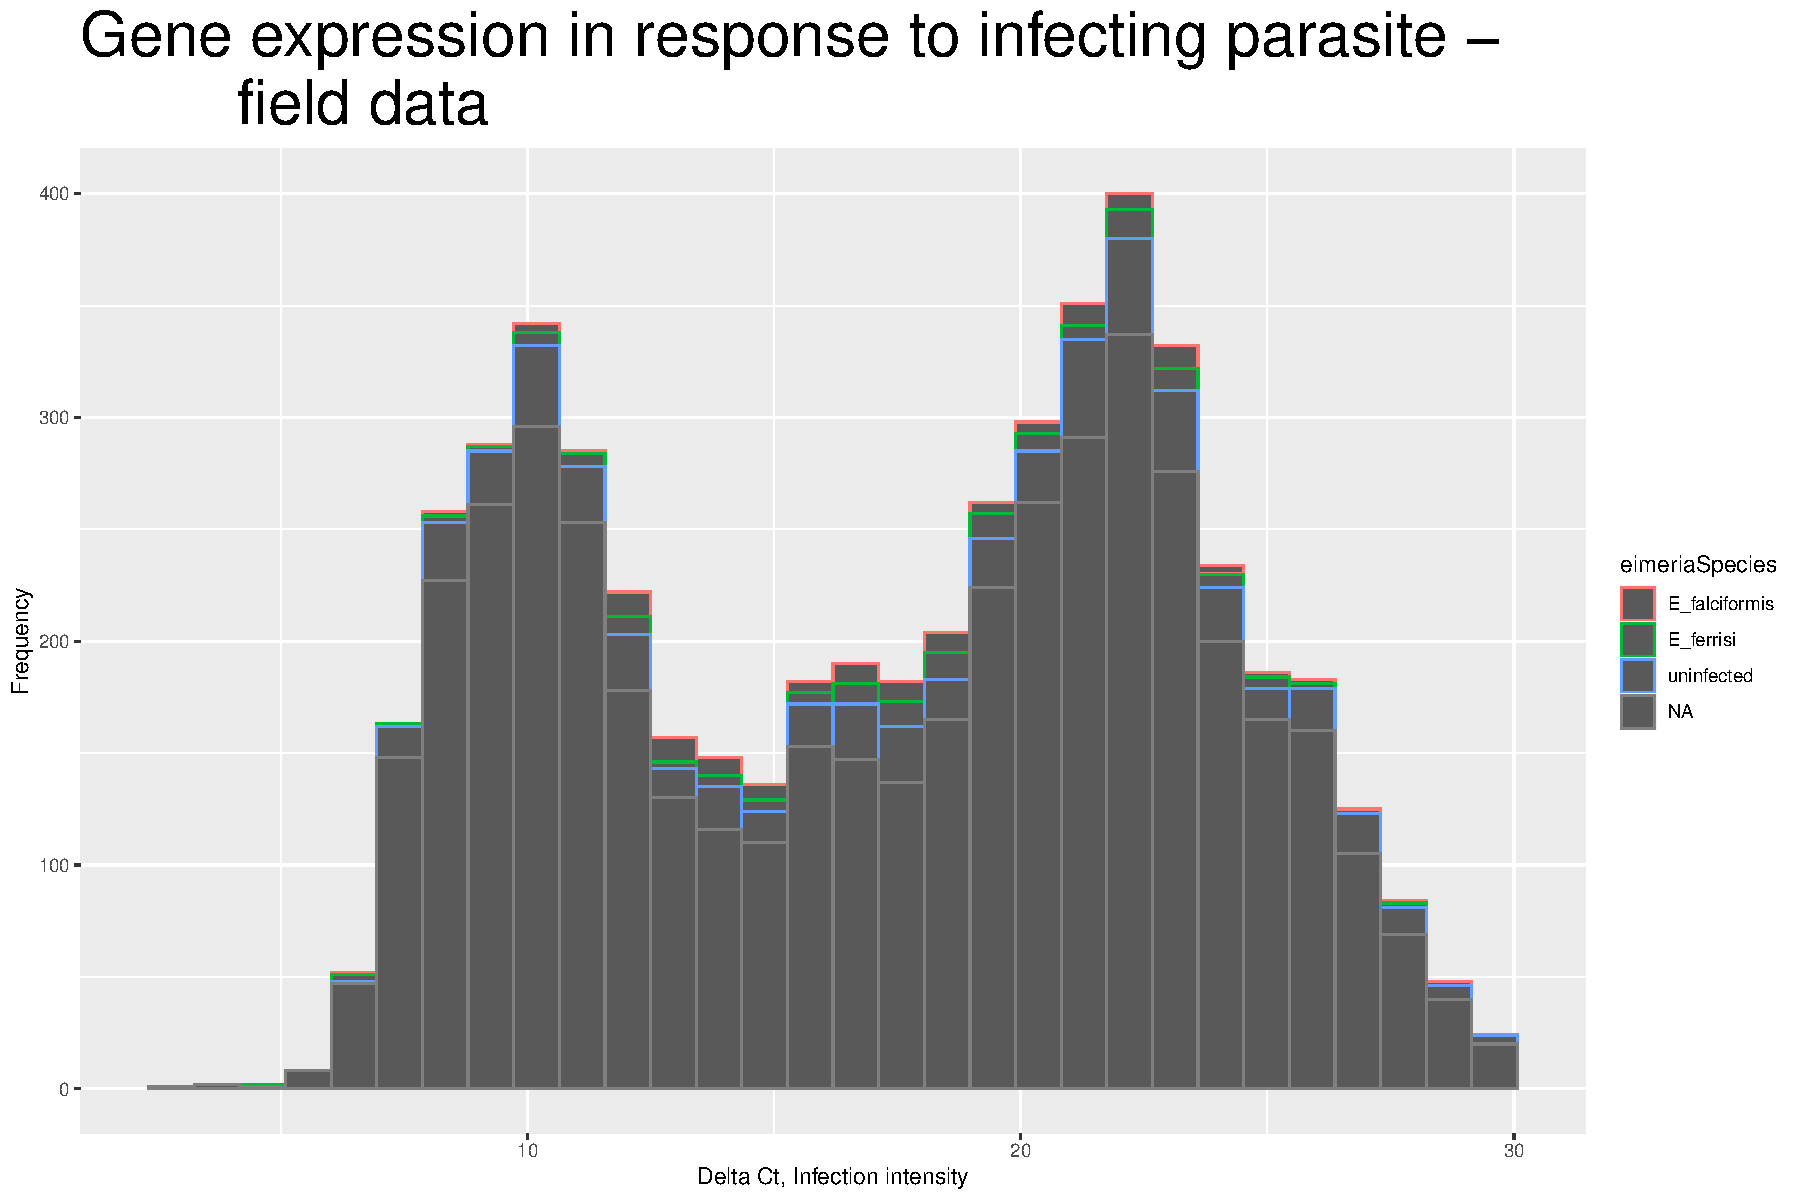
\includegraphics{1.Gene_expression_analysis_files/figure-latex/unnamed-chunk-9-1.pdf}

\begin{Shaded}
\begin{Highlighting}[]
\FunctionTok{write.csv}\NormalTok{(imputed\_expr, }\StringTok{"output\_data/gene\_expression/data\_products/imputed\_gene\_expression.csv"}\NormalTok{, }\AttributeTok{row.names =} \ConstantTok{FALSE}\NormalTok{)}

\FunctionTok{write.csv}\NormalTok{(g2, }\StringTok{"output\_data/gene\_expression/data\_products/clean\_gene\_expression.csv"}\NormalTok{, }\AttributeTok{row.names =} \ConstantTok{FALSE}\NormalTok{)}
\end{Highlighting}
\end{Shaded}


\end{document}
